\documentclass[10pt, pdf, hyperref={unicode},aspectratio=1610,clock, envcountsect]{beamer}

% Подключение пакета для поддержки русского языка 
\usepackage[russian]{babel}

% Использование пакета fontspec для настройки шрифтов 
\usepackage{fontspec} \setmainfont[Ligatures=TeX]{Times New Roman} \setsansfont[Ligatures=TeX]{Arial} \setmonofont{Courier New}
\usepackage{emoji}
\usepackage{caption}
\usepackage{algorithm2e}
% Определение темы Beamer (можно выбрать любую другую) 
\usepackage{amsmath,amssymb,amsfonts,amsthm,graphicx} 
\usetheme{Pittsburgh}
\usecolortheme{seagull}
\usepackage{tikz}
\usetikzlibrary{positioning, arrows.meta, shapes.geometric, fit}

% Определение стилей для узлов
\tikzset{
	theme/.style={rectangle, rounded corners=5pt, draw=black!50, thick, 
		fill=gray!15, text width=5.5cm, minimum height=1.0cm, 
		align=center, font=\Large\bfseries\sffamily, inner sep=8pt},
	class/.style={rectangle, draw=blue!70, thick, 
		fill=blue!10, text width=4.5cm, minimum height=0.8cm, 
		align=center, font=\normalsize\bfseries\sffamily, inner sep=5pt},
	subclass/.style={rectangle, draw=green!60!black, dashed, thin, 
		fill=green!10, text width=3.8cm, minimum height=0.7cm, 
		align=center, font=\footnotesize\sffamily, inner sep=4pt}
}


%\setbeamercovered{transparent} %Что это?
\setbeamertemplate{navigation symbols}{} % Что это?
\setbeamertemplate{theorems}[numbered]

%\setbeamercolor{block body}{fg=blue,bg=white}
\setbeamercolor{block body alerted}{bg=alerted text.fg!10}
\setbeamercolor{block title alerted}{bg=alerted text.fg!20}
\setbeamercolor{block body}{bg=structure!10}
\setbeamercolor{block title}{bg=structure!20}
\setbeamercolor{block body example}{bg=green!10}
\setbeamercolor{block title example}{bg=green!20}

\newtheorem{thm}{Теорема}
\newtheorem{lem}{Лемма}
\newtheorem{assert}{Утверждение}
\newtheorem{cor}{Следствие}

\theoremstyle{definition}
\newtheorem{df}{Определение}

\theoremstyle{remark}
\newtheorem{zam}{Замечание}
\newtheorem{con}{Condition}
\newtheorem{stm}{Statement}
\newtheorem{hpm}{Hypothesis}
\newtheorem{asm}{Предположение}
\newtheorem{ass}{Утверждение}
\newtheorem*{prb*}{Задача}

\newcommand{\doc}{\mbox{P r o o f}}
\newcommand{\frc}[2]{\scriptsize\raisebox{2pt}{$#1$}\big/\raisebox{-3pt}{$#2$}} 

\setbeamertemplate{footline}
{%
	\begin{beamercolorbox}{section in head/foot}
		\vskip2pt%
		\hbox to \paperwidth{ \insertnavigation{0.9\paperwidth}
			%\hfill \initclock \resetcrono
			%{\tiny \cronominutes \pdfcolon \cronoseconds}
			{\scriptsize \bfseries \insertframenumber}\hspace*{3mm}}%
		\vskip2pt
	\end{beamercolorbox}%
}

\DeclareCaptionLabelFormat{bf-parens}{Figure \textbf{#2}}
\captionsetup{labelformat = bf-parens, labelsep = endash}

\title{Об асимптотических свойствах множеств достижимости нелинейных систем в задачах управления с интегральными ограничениями}
\author{{И.\,О.~Осипов, \\
		{\small Диссертация на соискание ученой степени кандидата физико-математических наук}\\
{Научный руководитель: М.\,И.~Гусев}}}
\date{{Семинар кафедры теории управления и оптимизации ЧелГУ, \\ Челябинск, \\  12 февраля 2026 г.}}

\begin{document}
	\setemojifont{TwemojiMozilla}
	
	\begin{frame}[plain]
		\maketitle
	\end{frame}

\section{Введение}

\begin{frame}{Структура доклада}
	\begin{itemize}
		\item[\emoji{green-circle}] Введение
		\item[\emoji{green-circle}] Глава 1. Множества достижимости нелинейных систем с интегральными ограничениями
		\item[\emoji{green-circle}] Глава 2. Асимптотика множеств достижимости на малом интервале времени и синтез управлений
		\item[\emoji{green-circle}] Глава 3. Выпуклость множеств достижимости квазилинейных систем с интегральными ограничениями на управление
		\item[\emoji{green-circle}] Приложение. Численный метод построения множеств
		достижимости при интегрально-квадратичных ограничениях на управление
	\end{itemize}
\end{frame}

\begin{frame}{Об асимптотических свойствах множеств достижимости нелинейных систем в задачах управления с интегральными ограничениями}
	\begin{columns}
	\column{0.45\textwidth}
	\begin{itemize}
		\item[\emoji{green-circle}] Множества достижимости
		\item[\emoji{green-circle}] Ограничение на управление
		\begin{itemize}
			\item[\emoji{cross-mark}] Геометрические (мгновенные)
			\item[\emoji{check-mark}] Интегральные
			\begin{itemize}
				\item[\emoji{check-mark-button}] \underline{Квадратичные}
			\end{itemize}
		\end{itemize}
		\item[\emoji{green-circle}] Задачи с малым параметром
		\begin{itemize}
			\item[\emoji{cross-mark}] Сингулярные
			\item[\emoji{check-mark}] \underline{Регулярные}
		\end{itemize}
	\end{itemize}
		\column{0.45\textwidth}
				\begin{itemize}
			\item[\emoji{green-circle}]  Выпуклость множеств достижимости
				\item[\emoji{green-circle}] Линеаризация
					\item[\emoji{green-circle}] Квазилинейные системы
		\end{itemize}
	\end{columns}
\end{frame}

\begin{frame}{Множества достижимости (МД)}
	\begin{itemize}
		\item[\emoji{green-circle}] Анализ и синтез управляющий воздействий
		\begin{itemize}
			\item {\footnotesize Болтянский~В.\,Г., Гамкрелидзе~Р.\,В., Понтрягин~Л.\,С. Теория оптимальных процессов. I.~Принцип максимума~// Изв. АН СССР. Сер. матем. --- 1960.}
			\item {\footnotesize Беллман~Р. Динамическое программирование. --- М.: Изд-во иностр. лит., 1960.}
			\item {\footnotesize Lee~E.\,B., Markus~L. Foundations of Optimal Control Theory. --- New York~: John Wiley \& Sons, 1967.}
			\item {\footnotesize Красовский~Н.\,Н. Теория управления движением. --- М.: Наука, 1968.}
		\end{itemize}
		\item[\emoji{green-circle}] Анализ управляемости
		\begin{itemize}
			\item {\footnotesize Куржанский~А.\,Б. Управление и~наблюдение в~условиях неопределенности. --- М.: Наука, 1977. --- 392~с.}
			\item {\footnotesize Kurzhanski~A.\,B., Varaiya~P. Dynamics and Control of Trajectory Tubes. Theory and Computation. --- Birkhauser, 2014. --- 421~p.}
		\end{itemize}
		\item[\emoji{green-circle}] Анализ внешних возмущений, верификация и безопасное управление
		\begin{itemize}
			\item {\footnotesize Filippova~T.\,F., Matviychuk~O.\,G. Estimates of Reachable Sets of Control Systems with Bilinear--Quadratic Nonlinearities~// Ural Mathematical Journal. --- 2015.}
			\item {\footnotesize Mitchell~I.\,M., Bayen~A.\,M., Tomlin~C.\,J. A time-dependent Hamilton-Jacobi formulation of reachable sets for continuous dynamic games~// IEEE Transactions on Automatic Control. --- 2005.}
		\end{itemize}
		\item[\emoji{green-circle}] Задачи гарантированного оценивания и наблюдения  
		\begin{itemize}
			\item {\footnotesize Ананьев~Б.\,И. Об информационных множествах для многошаговых статистически неопределённых систем~// Тр. ИММ УрО РАН. --- 2000. --- Т.~6, №~2. --- С.~290--306.}
			\item {\footnotesize Schweppe~F.\,C. Uncertain Dynamic Systems. --- NJ~: Prentice-Hall, 1973. --- 563~p.}
		\end{itemize}
	\end{itemize}
\end{frame}

\begin{frame}{Интегральные ограничения на управление}
	\begin{itemize}{ \footnotesize
		\item Kurzhanski~A.\,B., Varaiya~P. Dynamics and Control of Trajectory Tubes. Theory and Computation. --- Birkhauser, 2014. --- 421~p.\\ https://people.eecs.berkeley.edu/~varaiya/Download/KurzhanskiVaraiya.pdf
		\item Polyak~B.\,T. Convexity of the reachable set of nonlinear systems under L2 bounded controls~// Dynam. Contin. Discrete Impuls. Systems Ser. A Math. Anal. --- 2004. --- Vol.~11, Suppl.~2-3. --- P.~255--267.
		\item Guseinov~K.\,G., Ozer~O., Akyar~E., Ushakov~V.\,N. The approximation of reachable sets of control systems with integral constraint on controls~// Nonlinear Differential Equations and Applications. --- 2007. --- Vol.~14, no.~1-2. --- P.~57--73.
		\item Huseyin~A., Huseyin~N., Guseinov~Kh.\,G. Continuity of Lp Balls and Application to the Nonlinear Control System~// Dynamic Systems: Stability, Control, Differential Games~: Proc. Int. Conf. devoted to the 100th anniversary of N.\,N.~Krasovskii (Yekaterinburg, Sept. 9--13, 2024). --- Yekaterinburg~: IMM UB RAS, 2024. --- P.~459--462.
		\item Gusev~M.\,I., Zykov~I.\,V. On Extremal Properties of the Boundary Points of Reachable Sets for Control Systems with Integral Constraints~// Proc. Steklov Inst. Math. --- 2018. --- Vol.~300. --- P.~114--125.
		\item Костоусова~Е.\,К. О полиэдральном оценивании множеств достижимости в~<<расширенном>> пространстве для многошаговых систем с~неопределенными матрицами и~интегральными ограничениями~// Тр. ИММ УрО РАН. --- 2020. --- Т.~26, №~1. --- С.~141--155.
		\item Пацко~В.\,С., Трубников~Г.\,И., Федотов~А.\,А. Множество достижимости машины Дубинса с~интегральным ограничением на управление~// Математическая теория игр и~eё приложения. --- 2023. --- Т.~15, №~2. --- С.~89--104.}
	\end{itemize}
\end{frame}

\begin{frame}{Выпуклость множеств достижимости}
	\begin{itemize}{ \footnotesize
	\item  Поляк~Б.\,Т. Локальное программирование~// Журнал вычислительной математики и~математической физики. --- 2001. --- Т.~41, №~9. --- С.~1324--1331.
	\item Ледяев~Ю.\,С. Критерии выпуклости замкнутых множеств в~банаховых пространствах~// Оптимальное управление и~дифференциальные уравнения~: сб. ст. к~110-летию со дня рождения акад. Л.\,С.~Понтрягина. --- М.: МИАН, 2019. --- (Тр. МИАН~; т.~304). --- С.~205--220. 
	\item Райсиг~Г. Выпуклость множеств достижимости систем управления~// Автоматика и~телемеханика. --- 2007. --- №~9. --- С.~64--78.}
	\end{itemize}
	Выпуклое МД существенно упрощает решение целого ряда задач:
	\begin{enumerate}
		\item Задачи минимизации выпуклых функционалов (время, энергия и т.д.).
		\item Задачи управляемости и достижимости. 
		\item Задачи синтеза управления. 
		\item Оценка и аппроксимация. 
	\end{enumerate}
		\begin{itemize}{ \footnotesize
			\item  Krener~A., Sch\"{a}ttler~H. The structure of small-time reachable sets in low dimensions~// SIAM J. Control Optim. --- 1989. --- Vol.~27, no.~1. --- P.~120--147. 
			\item Sch\"{a}ttler~H. Small-time reachable sets and time-optimal feedback control~// Nonsmooth Analysis and Geometric Methods in Deterministic Optimal Control. --- NY~: Springer, 1996. --- (The IMA Volumes in Mathematics and Its Applications~; vol.~78). --- P.~203--225. }
	\end{itemize}
\end{frame}

\begin{frame}{Квазилинейные системы}
			\begin{itemize}{ \footnotesize
			\item Киселёв~Ю.\,Н. Асимптотическое решение задачи оптимального быстродействия систем управления, близких к~линейным~// Докл. АН СССР. --- 1968. --- Т.~182, №~1. --- С.~31--34.
			\item Альбрехт~Э.\,Г. Об оптимальном управлении движением квазилинейных систем~// Дифференц. уравнения. --- 1969. --- Т.~5, №~3. --- С.~430--442.
			\item
			Альбрехт~Э.\,Г. О сближении квазилинейных объектов в~регулярном случае~// Дифференц. уравнения. --- 1971. --- Т.~7, №~7. --- С.~1171--1178.
			\item Dauer~J.\,P. Nonlinear perturbations of quasi-linear control systems~// Journal of Mathematical Analysis and Applications. --- 1976. --- Vol.~54, no.~3. --- P.~717--725. 
			\item Кремлев~А.\,Г. Об управлении квазилинейной системой при неопределенных начальных условиях~// Дифференц. уравнения. --- 1980. --- Т.~16, №~11. --- С.~1967--1979.
			\item Калинин~А.\,И., Лавринович~Л.\,И. Асимптотический метод минимизации интегрального квадратичного функционала на траекториях квазилинейной динамической системы~// Докл. Нац. акад. наук Беларуси. --- 2018. --- Т.~62, №~5. --- С.~519--524. 
			\item Габасов~Р.\,Ф., Калинин~А.\,И., Кириллова~Ф.\,М., Лавринович~Л.\,И. К асимптотическим методам оптимизации квазилинейных систем управления~// Тр. ИММ УрО РАН. --- 2019. --- Т.~25, №~3. --- С.~62--72.
			\item Ching~Sh., Eun~Yo., Gokcek~C., Kabamba~P., Meerkov~S. Quasilinear Control: Performance Analysis and Design of Feedback Systems with Nonlinear Sensors and Actuators. --- Cambridge University Press, 2010. --- 284~p.
			\item Guo~Y., Kabamba~P.\,T., Meerkov~S.\,M., Ossareh~H.\,R., Tang~C.\,Y. Quasilinear Control of Wind Farm Power Output~// IEEE Transactions on Control Systems Technology. --- 2015. --- Vol.~23, no.~4. --- P.~1555--1562.
			 }
	\end{itemize}
\end{frame}

\section{Глава 1}

\begin{frame}{Глава 1. Множества достижимости нелинейных систем с интегральными ограничениями}
	\begin{itemize}
		\item[\emoji{green-circle}] Некоторые свойства решений нелинейных систем с интегральными ограничениями
		\item[\emoji{green-circle}] Выпуклость множеств достижимости при малых ограничениях на управление
		\item[\emoji{green-circle}] Выпуклость множеств достижимости на малых интервалах времени
	\end{itemize}
\end{frame}

\begin{frame}{Общие предположения}
		Рассматривается нелинейная система, аффинная по управлению
		\begin{gather}\label{s1:common_nonlinear}
				\dot{x}(t)=f_1\big(t,x(t)\big)+f_2\big(t,x(t)\big)u(t), \qquad  t_0 \leqslant t \leqslant \overline{T}, \qquad x(t_0) = x_0.
		\end{gather}
		
		\begin{itemize}
			\item[\emoji{green-circle}] Функции $ f_1: [t_0, \overline{T}] \times \mathbb{R}^n \rightarrow \mathbb{R}^{n} $, $ f_2: [t_0, \overline{T}] \times \mathbb{R}^n \rightarrow \mathbb{R}^{n \times r} $ непрерывны по паре $(t,x)$ и непрерывно-дифференцируемы по $x$ в $ [t_0, \overline{T}] \times \Omega $, где $\Omega \subset \mathbb{R}^n$.
			\item[\emoji{green-circle}] $x_0 \in \Omega $.
			\item[\emoji{green-circle}]  $ u(\cdot) \in \mathbb{L}_2[t_0, \overline{T}] $.
		\end{itemize}
		
		\begin{asm}\label{s1:as:right_hand_side_conditions_global}
			Существует такое $\overline{\mu} > 0 $, что все решения (траектории) $ x(t, u(\cdot)) $ системы \eqref{s1:common_nonlinear}, отвечающие управлениям $u(\cdot) \in B_{\mathbb{L}_2[t_0, \overline{T}]}(0,\overline{\mu})$, определены на интервале $ [t_0,\overline{T}] $ и лежат в некотором выпуклом компакте $D \subset \Omega \subset \mathbb{R}^n$. 
		\end{asm}
		
		Далее, будем считать, что управление $ u(\cdot) \in B_{\mathbb{L}_2[t_0, \overline{T}]}(0,\mu) $, где $ 0 < \mu \leqslant \overline{\mu} $.
\end{frame}

\begin{frame}{Липшицевость решений по управлению}
	\begin{lem}\label{s1:lem:lip_of_solutions_global}
		Пусть выполнено Предположение \ref{s1:as:right_hand_side_conditions_global}.
		Тогда найдётся такое $L_x > 0$, что для любых $u_i(\cdot) \in B_{\mathbb{L}_2[t_0, \overline{T}]}(0,\mu) $, $i = 1,2$, и $t \in [t_0, \overline{T}]$
		\begin{gather*}
			\left\| x_1(t) - x_2(t) \right\| \leqslant L_x \left\|u_1(\cdot) - u_2(\cdot) \right\|_{\mathbb{L}_2[t_0, \overline{T}]}, 
		\end{gather*}
		где $x_i(t) = x_i(t,u_i(\cdot))$, $i = 1,2$. 
	\end{lem}
	Константа $L_x$ выбрана не зависящей от $t$, таким образом
	\begin{gather*}
		\left\| x_1(\cdot) - x_2(\cdot) \right\|_{\mathbb{C}[t_0, \overline{T}]} \leqslant L_x \left\|u_1(\cdot) - u_2(\cdot) \right\|_{\mathbb{L}_2[t_0, \overline{T}]}.
	\end{gather*}
\end{frame}

\begin{frame}
	\begin{df}\label{s1:def:linearized_system}
		Пусть $ x(\cdot,u(\cdot)) $ ~--- движение, отвечающее управлению $ u(\cdot)$.
		Назовём систему
		\begin{gather}\label{s1:linearized_system}
			\delta \dot{x} = A(t) \delta x + B(t) \delta u, \qquad t_0 \leqslant t \leqslant T, \qquad \delta x(t_0) = 0,
		\end{gather}
		линеаризацией системы \eqref{s1:common_nonlinear} вдоль пары траектории и управления $\left( x(\cdot,u(\cdot)),u(\cdot)\right) $, если 
		\begin{gather*}
			A(t) = \dfrac{\partial f_1}{\partial x} \Big(t,x\big(t,u(\cdot)\big)\Big) 
			+ 
			\sum\limits_{k = 1}^{r}
			\dfrac{\partial f_2^k}{\partial x}\Big(t,x\big(t,u(\cdot)\big)\Big) u^k(t), \ 
			B(t) = f_2 \Big(t,x\big(t,u(\cdot)\big)\Big).
		\end{gather*}
		Здесь $ A(\cdot) $ представляет собой матрицу Якоби функции $ f_1(\cdot, x) + f_2(\cdot, x) u(\cdot) $, вычисленную вдоль траектории $ x(\cdot,u(\cdot)) $.
	\end{df}
\end{frame}

\begin{frame}
	Введём отображение $F: \mathbb{L}_2 \rightarrow \mathbb{R}^n $
	\begin{gather}\label{s1:solution_endpoint_mapping}
		F(u(\cdot)) = x(T,u(\cdot)), \qquad 0 \leqslant T \leqslant \overline{T}.
	\end{gather} 
	\begin{lem}\label{s1:lem:frechet_derivative_common}
		Пусть выполнено Предположение \ref{s1:as:right_hand_side_conditions_global}.
		Тогда отображение $F$ имеет непрерывную производную Фреше, определяемую равенством $ F'(u(\cdot))\delta u(\cdot) =\delta x(T)$, где $\delta x(T)$ ~--- решение линеаризованной вдоль пары $\left( x(t,u(\cdot)),u(\cdot)\right) $ системы \eqref{s1:linearized_system}, порождённое управлением $\delta u(\cdot)$ при нулевом начальном условии.
	\end{lem}
	\begin{gather}\label{s1:lem2_assert}
		F'(u(\cdot))\delta u(\cdot) =\delta x(T) = \int\limits_{t_0}^{T} X(T, \tau) B(\tau) \delta u(\tau) \ d\tau.
	\end{gather}
\end{frame}

\begin{frame}
	\begin{df}
		Множеством достижимости $ G(T,\mu) $ системы \eqref{s1:common_nonlinear} в пространстве состояний в момент времени $ T $ назовём множество всех концов траекторий $ x(T, u(\cdot)) \in \mathbb{R}^n $, которые могут быть порождены управлениями $ u(\cdot) \in B_{\mathbb{L}_2}(0,\mu) =\left\lbrace u:\lVert u(\cdot)\rVert^2_{\mathbb{L}_2} \leqslant \mu^2\right\rbrace $,
		\begin{gather*}
			G(T,\mu)=\{x\in \mathbb{R}^n:\exists u(\cdot)\in B_{\mathbb{L}_2}(0,\mu),\; x=x(T,u(\cdot))\}.
		\end{gather*}
	\end{df}
	$G(T,\mu)$ есть образ гильбертова шара $B_{\mathbb{L}_2}(0,\mu)$ при его отображении $F$.
	\begin{df}
		Линейная система $\dot{y} = A(t) y + B(t) u $ называется управляемой (вполне управляемой) на интервале времени $ t_0 \leqslant t \leqslant T $, если для любых $y_0, y_1 \in \mathbb{R}^n$ найдётся управление $u(\cdot) \in \mathbb{L}_2$, переводящее систему из $y(0, u(\cdot)) = y_0 $ в $y(T, u(\cdot)) = y_1 $.
	\end{df}
\end{frame}

\begin{frame}
		\begin{df}\label{s1:def:grammian}
		Симметричная матрица, определённая равенством
		\begin{gather*}
			W(T) = \int\limits_{t_0}^{T}X(T,t)B(t)B^{\top}(t)X^{\top}(T,t) \, dt,
		\end{gather*}
		называется грамианом управляемости линейной системы $\dot{y} = A(t) y + B(t) u $ на интервале времени $ t_0 \leqslant t \leqslant T $.
		Как и в Определении \ref{s1:def:linearized_system}, здесь $ X(\tau_1,\tau_0)= \Phi(\tau_1) \Phi^{-1}(\tau_0) $, где $\Phi(t) $ ~--- фундаментальная матрица решений однородной системы, удовлетворяющая уравнению $ \dot{\Phi}(t) = A(t) \Phi(t)$, $ \Phi(t_0) = I $.
	\end{df}
	\begin{itemize}
		\item[\emoji{green-circle}] Линейная система вполне управляема на $ [t_0, T] $ \Leftrightarrow $W(T) \succ 0 $.
		\item[\emoji{green-circle}] $W(T,u(\cdot))$ --- грамиан управляемости системы \eqref{s1:linearized_system}.  $W(T,u(\cdot))\succ 0 $ \Rightarrow регулярность $F$ в точке $u(\cdot) $.
	\end{itemize}
\end{frame}

\begin{frame}{Выпуклость отображения малого шара}
	Пусть $X$, $Y$ --- два гильбертовых пространства, а $f:X\to Y$ --- нелинейное отображение с производной Фреше на шаре $B(a, r) =\{x\in X:\|x - a\| \leqslant r\}$.
	
%	\begin{gather}
%		\|f'(a)∗y\| \geqslant \nu\|y\|, \qquad \forall y \in Y.
%	\end{gather}
	\begin{thm}[\footnote{Polyak~B.\,T. Convexity of Nonlinear Image of a Small Ball with Applications to Optimization. Set-Valued Analysis, 2001, Vol. 9, P. 159–168.}\label{s1:th:PolyakTh}]
		Пусть $a \in X$~--- регулярная точка отображения $f: X \rightarrow Y$, производная Фреше $f'$ существует и удовлетворяет условию Липшица на шаре $B_X(a,r) $, $r > 0$ c константой $ L > 0 $, а также выполнено условие
		\begin{gather*}
			\varepsilon < \min\left\{r,\frac{\nu}{2L}\right\},
		\end{gather*}
		где $\nu$~--- наименьшее сингулярное число отображения $f'(a)$.
		Тогда образ шара $B_X(a,\varepsilon) $ при отображении $f$ является выпуклым, т.~е. $F = \{f(x): x \in B_X(a,\varepsilon)\}$~--- выпуклое множество в $Y$.
		Более того, это множество сильно выпуклое и его граница состоит из образов граничных точек шара: $\partial F \subset f(\partial B_X(a,\varepsilon))$.
	\end{thm}
\end{frame}

\begin{frame}
	\begin{asm}\label{s1:as:right_hand_side_diff_lip}
		Функции $f_1(t,x)$ и $f_2(t,x)$ имеют производные по $x$, которые удовлетворяют условию Липшица при всех $t \in [t_0;T]$, $x_1, x_2 \in D$:
		\begin{gather*}
			\left\| \frac{\partial f_1}{\partial x}(t,x_1) - \frac{\partial f_1}{\partial x}(t,x_2) \right\| \leqslant l_{f_1} \| x_1 - x_2\|, \quad \left\| \frac{\partial f_2^k}{\partial x}(t,x_1) - \frac{\partial f_2^k}{\partial x}(t,x_2) \right\| \leqslant l_{f_2^k} \| x_1 - x_2\|,
		\end{gather*}
		где $l_{f_1} > 0$ и $l_{f_2^k} > 0$, $k = 1,...,r$.
	\end{asm}
	\setcounter{lem}{3}
	\begin{lem}\label{s1:lem:lip_dx_global}
		Пусть выполнены Предположения \ref{s1:as:right_hand_side_conditions_global} и \ref{s1:as:right_hand_side_diff_lip}.
		Тогда найдётся константа $L_u > 0$ такая, что для всех $u_1(\cdot),\, u_2(\cdot) \in B_{\mathbb{L}_2}(0,\mu)$ и $t \in [t_0,T]$ выполнено неравенство 
		\begin{gather*}
			\Big\| F'(u_1(\cdot)) - F'(u_2(\cdot)) \Big\|_{\mathcal{L}(\mathbb{L}_2, \mathbb{R}^n)} \leqslant L_u \| u_1(\cdot) - u_2(\cdot) \|_{\mathbb{L}_2}.
		\end{gather*}
		Здесь $\mathcal{L}(\mathbb{L}_2, \mathbb{R}^n)$ --- пространство линейных ограниченных операторов, действующих из $\mathbb{L}_2$ в $\mathbb{R}^n$, а \mbox{$\| \cdot \|_{\mathcal{L}(\mathbb{L}_2, \mathbb{R}^n)}$} --- операторная норма. 
		Для некоторого оператора $T: \mathbb{L}_2 \to \mathbb{R}^n $, $\| T \|_{\mathcal{L}(\mathbb{L}_2, \mathbb{R}^n)} = \sup\limits_{\|x\|_{\mathbb{L}_2} = 1} \| T x \| $.
	\end{lem}
\end{frame}

\begin{frame}{Выпуклость множеств достижимости при малых ограничениях на управление}
	\begin{thm}[\footnote{Polyak~B.\,T. Convexity of the reachable set of nonlinear systems under L2 bounded controls~// Dynam. Contin. Discrete Impuls. Systems Ser. A Math. Anal. --- 2004. --- Vol.~11, Suppl.~2-3. --- P.~255--267.}]\label{s1:th:small_control_convexity}
		Пусть выполнены Предположения \ref{s1:as:right_hand_side_conditions_global} и \ref{s1:as:right_hand_side_diff_lip}, и пусть линеаризованная вдоль пары $\left( x(\cdot,0),0\right) $ система \eqref{s1:common_nonlinear} является управляемой.
		Тогда найдётся такое $\mu_0 > 0$, что при всех $0 < \mu < \mu_0 $ множества достижимости $G(T, \mu)$ системы \eqref{s1:common_nonlinear} будут выпуклыми.
	\end{thm}
	\begin{gather}\label{s1:mu0}
		\mu_0 = \min\left( \dfrac{\sqrt{\lambda\big(W(T,0)\big)}}{2L_u}, \overline{\mu} \right).
	\end{gather}
\end{frame}

\begin{frame}{Выпуклость множеств достижимости на малых интервалах времени}
	Рассмотрим нелинейную систему \eqref{s1:common_nonlinear} на малом интервале времени $\ t_0 \leqslant t \leqslant t_0 + \overline{\varepsilon} $
	\begin{gather}\label{s1:common_nonlinear_small_time}
		\dot{x}(t)=f_1(t,x(t))+f_2(t,x(t))u(t), \qquad x(t_0) = x_0, \qquad \overline{\varepsilon} > 0.
	\end{gather}
	\begin{gather*}
		\lVert u(\cdot)\rVert^2_{\mathbb{L}_2[t_0,t_0+\overline{\varepsilon}]}  \leqslant \mu^2.
	\end{gather*}
	
	Пусть $ 0 < \varepsilon \leqslant \overline{\varepsilon} $.
	
	С учетом замены времени $ t = \varepsilon \tau + t_0 $ и обозначений $ z(\tau) = x(\varepsilon \tau + t_0) $ и $ \upsilon(\tau) = \varepsilon u(\varepsilon \tau + t_0) $
	\begin{gather}\label{s1:eps_nonlinear}
		\dot{z}(\tau)=\widetilde{f}_1(\tau,z(\tau))+\widetilde{f}_2(\tau,z(\tau))\upsilon(\tau), \qquad 0 \leqslant \tau \leqslant 1, \qquad z(0) = x_0,
	\end{gather}
	где $ \widetilde{f}_1(\tau,z) = \varepsilon f_1(\varepsilon \tau + t_0,z) $, $ \widetilde{f}_2 (\tau,z) = f_2(\varepsilon \tau + t_0,z)$, а управление $ \upsilon(\cdot) $ удовлетворяет ограничению
	\begin{gather*}%\label{s1:eps_control_constaint}
		\int_0^1 \upsilon^{\top}(\tau) \upsilon(\tau) \, d\tau \leqslant \left( \mu \sqrt{\varepsilon}\right)^2.
	\end{gather*}
\end{frame}

\begin{frame}
	\begin{itemize}
		\item[\emoji{green-circle}] Для системы \eqref{s1:eps_nonlinear} выполняется Предположение \ref{s1:as:right_hand_side_conditions_global} в области $[0, 1]\times D$ и $\upsilon(\cdot) \in B_{\mathbb{L}_2}(0, \overline{\mu}\sqrt{\varepsilon}) $ и Лемма \ref{s1:lem:lip_of_solutions_global}.
		\item[\emoji{green-circle}]  $G_{\varepsilon}(\tau) = \{z\in \mathbb{R}^n:\exists \upsilon(\cdot)\in \mathbb{L}_2, \lVert \upsilon(\cdot)\rVert_{\mathbb{L}_2}	\leqslant \mu \sqrt{\varepsilon}, \; z=z(\tau, \upsilon(\cdot))\}.$
		\item[\emoji{green-circle}] Линеаризуем \eqref{s1:eps_nonlinear} вдоль траектории $ z(\cdot,0) = x(\cdot, 0) $
		\begin{gather}\label{s1:eps_linearized}
			\delta\dot{z} = \widetilde{A}_{\varepsilon}(\tau, 0) \delta z(\tau) +\widetilde{B}_{\varepsilon}(\tau, 0) \delta \upsilon(t),\qquad 0 \leqslant \tau \leqslant 1, \qquad \delta z(0) = 0,
		\end{gather}
		где $ \widetilde{A}_{\varepsilon}(\tau, \upsilon(\cdot)) = \varepsilon A(\varepsilon \tau + t_0, u(\cdot)) $, $\widetilde{B}_{\varepsilon}(\tau, \upsilon(\cdot)) = B(\varepsilon \tau + t_0, u(\cdot)) $. 
		\item[\emoji{green-circle}]  Выполняются равенства
			$G_{\varepsilon}(1) = G(t_0 + \varepsilon) $ и $
			W_{\varepsilon} = \dfrac{1}{\varepsilon} W(t_0+\varepsilon, 0)$
		\item[\emoji{green-circle}] Отображение $S: \mathbb{L}_2[0,1] \rightarrow \mathbb{R}^n $, $S(\upsilon(\cdot)) = z(1,\upsilon(\cdot))$. 
		\item[\emoji{green-circle}] $ S'(\upsilon(\cdot))\delta \upsilon(\cdot) = \delta z(1) = \int\limits_0^1 X_{\varepsilon}(1, \tau, \upsilon(\cdot)) \widetilde{B}_{\varepsilon}(\tau, \upsilon(\cdot)) \delta\upsilon(\tau)\ d\tau$.
		\item[\emoji{green-circle}] Функции $\widetilde{f}_1$ и $\widetilde{f}_2$ удовлетворяют Предположению \ref{s1:as:right_hand_side_diff_lip} на множестве $[0, 1]\times D$, а отображение $S'(\upsilon)$ удовлетворяет условию Липшица с константой $L_u(\varepsilon)$.
	\end{itemize}
\end{frame}

\begin{frame}
	Так как $S'(0)S'(0)^* = W_{\varepsilon}$, то 
	\begin{itemize}
		\item[\emoji{green-circle}]  $ \lambda(\varepsilon) > 0 $ \Rightarrow регулярность отображения $S$ при $\upsilon = 0$.
		\item[\emoji{green-circle}]  $G_{\varepsilon}$ есть образ гильбертова шара $B_{\mathbb{L}_2}(0,\mu\sqrt{\varepsilon})$ при его отображении $S$.
	\end{itemize}
	\begin{thm}[\footnote{Gusev~M.\,I. Estimates of the minimal eigenvalue of the controllability Gramian for a system containing a small parameter~// Mathematical Optimization Theory and Operations Research. MOTOR 2019. --- Springer, Cham, 2019. --- (Lecture Notes in Computer Science~; vol.~11548). --- P.~383--395.}]\label{s1:th:small_time_convexity}
		Если найдутся такие $K > 0$, $ \alpha > 0$, $ 0 < \varepsilon_0 < \overline{\varepsilon}$, что для всех $\varepsilon \leqslant \varepsilon_0$ выполняется условие
		\begin{gather}\label{s1:small_time_convexity_condition}
			\lambda(\varepsilon) \geqslant \left\{ {\begin{array}{*{20}{l}}
					{K\varepsilon ^{3 - \alpha}, \mbox{\ если \ } f_2(t,x) \mbox{\ не зависит от \ } x}, \\
					{K\varepsilon ^{1 - \alpha}}, \mbox{\ в противном случае},
			\end{array}} \right.
		\end{gather}
		то существует такое $ \varepsilon_1 > 0 $, что множество достижимости $G(\varepsilon)$ системы \eqref{s1:common_nonlinear_small_time} выпукло при всех $\varepsilon < \varepsilon_1 $.
	\end{thm}
	Для проверки условия \ref{s1:small_time_convexity_condition} можно использовать разложение
	\begin{gather}\label{s1:gram1}
		W_{\varepsilon} = U_0 + \dfrac{\varepsilon}{2}U_1 + \dfrac{\varepsilon^2}{6} U_2 + \dfrac{\varepsilon^3}{24}U_3 + \dfrac{\varepsilon^4}{120}U_4 + \dots + \dfrac{\varepsilon^k}{(k+1)!}U_k + \dots,
	\end{gather}
	где $U_0 = B B^T$ и $		U_i = A U_{i-1} + U_{i-1} A^T, \ i \geqslant 1$.
\end{frame}

\section{Глава 2}

\begin{frame}{Глава 2. Асимптотика множеств достижимости на малом интервале времени и синтез управлений}
	\begin{itemize}
		\item[\emoji{green-circle}] Расстояние Банаха--Мазура и асимптотическая эквивалентность множеств
		\item[\emoji{green-circle}] Асимптотика множеств достижимости нелинейных систем с интегральными ограничениями
		\item[\emoji{green-circle}] Условие применимости метода линеаризации в задаче локального синтеза
	\end{itemize}
\end{frame}

\begin{frame}{Расстояние Банаха-Мазура}
	Пусть $ X, Y \subset \mathbb R^n $ --- выпуклые компакты, такие, что $0\in \mathrm{int}X$, $0\in \mathrm{int}Y$.\\
	Расстояние Банаха-Мазура $ \rho (X, Y) $ между $ X $ и $ Y $ определяется равенством
	$$ \rho (X, Y): = \log (r(X,Y) \cdot r(Y, X)),$$ где $r(X, Y) = \inf \{t \geqslant 1: tX \supset Y \}$.\\
	Справедливо
	$$r(X,Y) = \max \left\lbrace 1, \sup_{\| y \| = 1} \frac {\delta (y|X)}{\delta (y|Y)} \right\rbrace ,$$
	 где $ \delta(y|M) $ --- опорная функция множества M.
	$$r(sX,sY)=r(X,Y),\;\rho(sX,sY)=\rho(X,Y),\;s>0 $$
	Расстояние Банаха-Мазура инвариантно к масштабу множеств.
\end{frame}

\begin{frame}{Асимптотическая эквивалентность множеств}
	Пусть $ X=X(\varepsilon), Y=Y(\varepsilon) $ --- выпуклые компакты, и $0\in \mathrm{int}X(\varepsilon)$, $0\in \mathrm{int}Y(\varepsilon)$ при $ 0 <\varepsilon \leqslant\varepsilon_0 $.
	\begin{df}Множества $ X (\varepsilon), Y (\varepsilon) $ асимптотически эквиваленты\footnote[1]{Goncharova~E.,  Ovseevich~A. Small-time reachable sets of
			linear systems with integral control constraints: birth of the
			shape of a reachable set // Journal of Optimization Theory and
			Applications. 2016. Vol.~168. no.~2. pp.~615--624.}  если
		$$ \rho (X (\varepsilon), Y (\varepsilon)) \to 0,\;\; \varepsilon \to 0. $$ 
	\end{df}
	\vspace{0.1cm}
	Из $ \rho (X (\varepsilon), Y (\varepsilon)) \to 0 $ следует $ h(X (\varepsilon), Y (\varepsilon)) \to 0$, $\varepsilon\to 0$.\\
	\vspace{0.1cm}
	Обратное не верно:\\
	\vspace{0.1cm}
	Пусть $X(\varepsilon)=\{x\in \mathbb R^2: |x_1|\leqslant\varepsilon,\,|x_2|\leqslant\varepsilon \}$, $Y(\varepsilon)=\{x\in \mathbb R^2: x_1^2+x_2^2 \leqslant\varepsilon^2 \}$.\\
	\vspace{0.2cm}
	Тогда $h(X(\varepsilon), Y(\varepsilon))=(\sqrt{2}-1)\varepsilon\to 0$, и
	$\rho(X(\varepsilon), Y(\varepsilon))=\log \sqrt{2}>0 $.\\
\end{frame}


\begin{frame}{Достаточное условие асимптотической эквивалентности}
	\begin{thm}\label{suff}
		Пусть выполнены условия
		\begin{gather*}
			\lim\limits_{\varepsilon \rightarrow 0}h(X(\varepsilon),Y(\varepsilon)) = 0, \qquad \lim\limits_{\varepsilon \rightarrow 0}\frac{h(X(\varepsilon),Y(\varepsilon))}{\delta_{\min}(Y(\varepsilon))} = 0.
		\end{gather*}
		Тогда множества $ X(\varepsilon) $ и $ Y(\varepsilon) $\---~асимптотически эквивалентны.  Здесь \\ $ \delta_{\min}(Y(\varepsilon)) = \inf\limits_{\left\|y \right\| =1 } \delta(y|Y(\varepsilon))$.
	\end{thm}
\end{frame}


\begin{frame}{Условие асимптотической эквивалентности МД нелинейной и линеаризованной систем }
	\begin{gather}\label{s2:nonlinear_with_output}
		\begin{gathered}
			\dot{x}(t)=f_1(t,x(t))+f_2(t,x(t))u(t), \qquad t_0 \leqslant t \leqslant t_0 + \overline{\varepsilon}, \qquad x(t_0) = x_0, \\
			y(t) = C x(t).
		\end{gathered}
	\end{gather}
	$x\in \mathbb{R}^n$, $u\in \mathbb{R}^r$, $ y \in \mathbb{R}^m(m \leqslant n) $, $ C \in \mathbb{R} ^{m \times n}$, $ \mathrm{rank}(C) = m $, $ \overline{\varepsilon} > 0 $.\\
	Предположения \ref{s1:as:right_hand_side_conditions_global} и \ref{s1:as:right_hand_side_diff_lip} относительно функций $f_1$ и $f_2$ будем считать справедливыми на интервале $t_0 \leqslant t \leqslant t_0 + \overline{\varepsilon} $ при управлениях $u(\cdot) \in B_{\mathbb{L}_2}(0, \overline{\mu}) $, $\overline{\mu} > 0$.
	Пусть $ 0 < \varepsilon \leqslant \overline{\varepsilon} $. 
	\begin{gather*}
		G(\varepsilon)=\{x\in \mathbb{R}^n:\exists u(\cdot)\in B_{\mathbb{L}_2}(0,\mu),\; x=x(t_0+\varepsilon, u(\cdot))\}.
	\end{gather*}
	\begin{df}
		Множеством достижимости $\overline{G}(\varepsilon)$ системы \eqref{s2:nonlinear_with_output} по выходу $ y = C x $ будем называть множество всех выходов $ y(t_0+\varepsilon) $, соответствующих концам траекторий $ x(t_0+\varepsilon, u(\cdot)) $, порождённых управлениями $ u(\cdot) \in B_{\mathbb{L}_2}(0,\mu)$:
		\begin{gather*}
			\overline{G}(\varepsilon)=\{y\in \mathbb{R}^m:\exists u(\cdot)\in B_{\mathbb{L}_2}(0,\mu),\; y=Cx(t_0+\varepsilon, u(\cdot))\}.
		\end{gather*}
		 $ \overline{G}(\varepsilon) = C G(\varepsilon) $. 
	\end{df}
\end{frame}

\begin{frame}
\begin{df}
	Симметричная матрица, определённая равенством
	\begin{gather*}
		\overline{W}(t_0 + \varepsilon) = \int_{t_0}^{t_0+\varepsilon} C X(t_0+\varepsilon,t)B(t)B^{\top}(t)X^{\top}(t_0+\varepsilon,t) C^\top \, dt=CW(\varepsilon)C^\top,
	\end{gather*}
	называется грамианом управляемости линейной системы 
	\begin{gather}\label{s2:linear_system}
		\dot{s} = A(t) s + B(t) u
	\end{gather}
	на интервале времени $ t_0 \leqslant t \leqslant t_0 + \varepsilon $ по выходу $y = C s$. 
\end{df}
	По аналогии с \eqref{s1:eps_nonlinear} произведём замену времени $t = \varepsilon \tau + t_0$, примем обозначения $z(\tau) = x(\varepsilon \tau + t_0)$, $ \upsilon(\tau) = \varepsilon u(\varepsilon \tau + t_0) $, $h(\tau) = y(\varepsilon \tau + t_0)$ и получим из \eqref{s2:nonlinear_with_output}
	\begin{gather}\label{s2:eps_nonlinear_with_output}
		\begin{gathered}
			\dot{z}(\tau)=\widetilde{f}_1(\tau,z(\tau))+\widetilde{f}_2(\tau,z(\tau))\upsilon(\tau), \qquad 0 \leqslant \tau \leqslant 1, \qquad z(0) = x_0, \\
			h(\tau) = C z(\tau).
		\end{gathered}
	\end{gather}
	Здесь $ \widetilde{f}_1(\tau,z) = \varepsilon f_1(\varepsilon \tau + t_0, z) $, $ \widetilde{f}_2 (\tau,z) = f_2(\varepsilon \tau + t_0,z)$, а управление \mbox{$ \upsilon(\cdot) \in B_{\mathbb{L}_2}(0, \mu\sqrt{\varepsilon})$}.
\end{frame}

\begin{frame}
	 $\overline{G}_{\varepsilon}(\tau)$ --- множество достижимости системы \eqref{s2:eps_nonlinear_with_output} по выходу $h$ в момент времени $\tau$:
	Линеаризация системы \eqref{s2:eps_nonlinear_with_output} вдоль пары $(z(\cdot, 0), 0)$:
	\begin{gather}\label{s2:eps_linearized}
		\begin{gathered}
			\delta\dot{z} = A_{\varepsilon}(\tau) \delta z(\tau) + B_{\varepsilon}(\tau) \delta \upsilon(t),\qquad 0 \leqslant \tau \leqslant 1, \qquad \delta z(0) = 0, \\
			\delta h(\tau) = C \delta z(\tau).
		\end{gathered}
	\end{gather}
	Здесь $ A_{\varepsilon}(\tau) = \widetilde{A}_{\varepsilon}(\tau, 0) $ и  $B_{\varepsilon}(\tau) = \widetilde{B}_{\varepsilon}(\tau, 0) $.
	
	Кроме отображения  $S: \mathbb{L}_2[0,1] \rightarrow \mathbb{R}^n $, $S\upsilon(\cdot) = z(1,\upsilon(\cdot))$ определим еще отображение $ H: \mathbb{L}_2[0,1] \rightarrow \mathbb{R}^m $,  $ H(\upsilon(\cdot)) = C S(\upsilon(\cdot)) = C z(1,\upsilon(\cdot)) $.
	
	Отображение $ H $ непрерывно дифференцируемо по Фреше при всех $ \upsilon(\cdot) \in B_{\mathbb{L}_2[0,1]}(0,\sigma(\varepsilon)) $, и его производная Фреше $ H': \mathbb{L}_2[0,1] \rightarrow \mathbb{R}^m $ определена равенством
	\begin{gather*}
		H'( \upsilon(\cdot))\delta \upsilon = C S'(\upsilon(\cdot))\delta \upsilon = C \delta z(1) = \delta h(1) = C \int\limits_0^1 X_{\varepsilon}(1,\tau, \upsilon(\cdot)) \widetilde{B}_{\varepsilon} (\tau, \upsilon(\cdot)) \delta \upsilon(\tau) \ d \tau,
	\end{gather*}
	Управляемость системы \eqref{s2:eps_linearized} по выходу $\delta h$ ($\overline{W}_{\varepsilon} \succ 0 $, то есть $\overline{\lambda}(\varepsilon) > 0$), означает регулярность отображения $H$ в точке $\upsilon = 0$.
\end{frame}


\begin{frame}{Асимптотика множеств достижимости по выходу}
	\begin{thm}\label{s2:th:assimptotic_equality}
		При достаточно малых $ \varepsilon $ множество достижимости $ \overline{G}(\varepsilon) $ системы \eqref{s2:nonlinear_with_output} по выходу $ y = C x $ выпукло и асимптотически эквивалентно множеству \\ \mbox{$\overline{W}^{1/2}_{\varepsilon}B_{\mathbb{R}^m}(0,\mu) + Cx(t_0+\varepsilon,0)$}, если найдутся такие $ K>0 $, $ \alpha > 0 $, $ 0< \varepsilon_0<\overline{\varepsilon} $, что для всех $ \varepsilon \leqslant \varepsilon_0 $
		\begin{gather}\label{s2:cond1}
			\overline{\lambda}(\varepsilon) \geqslant \left\{ {\begin{array}{*{20}{l}}
					{K\varepsilon ^{3 - \alpha}, \mbox{\ если \ } f_2(t,x) \mbox{\ не зависит от \ } x}, \\
					{K\varepsilon ^{1 - \alpha}}, \mbox{\ в противном случае}.
			\end{array}} \right.
		\end{gather}
	\end{thm}
\end{frame}

\begin{frame}
	\begin{ass}
		 Пусть $ W_1 $, $ W $ --- симметричные матрицы, причём $ W_1 = C W C^{\top} $, где $ C $ --- матрица полного ранга размерности $ m \times n $, $ m \leqslant n $, а $ \nu(W) $, $ \nu(W_1) $ и $ \nu(CC^{\top}) $ --- наименьшие собственные числа соответствующих матриц.
		
		Тогда
		\begin{gather*}
			\nu(W_1) \geqslant \nu(CC^{\top}) \nu(W).
		\end{gather*}
	\end{ass}
	 Применяя утверждение к грамианам $ W_{\varepsilon} $ и $ \overline{W}_{\varepsilon}$, получим
	\begin{gather*}
		\overline{\lambda}(\varepsilon) \geqslant \nu(CC^{\top}) \lambda(\varepsilon),
	\end{gather*}
	где $ \nu(CC^{\top}) $ не зависит от $ \varepsilon $. 
	
	Если множество $ G(\varepsilon) $ --- выпуклое, то и для всех возможных матриц полного ранга $ C $, множества $ \overline{G}(\varepsilon) $ --- выпуклы. 
	
	Однако невыпуклое $ G(\varepsilon) $ может иметь выпуклые проекции.
\end{frame}


\begin{frame}
	\frametitle{Пример: Уницикл}
	Рассмотрим систему \footnote{Patsko V.S., Fedotov A.A. Attainability Set at Instant for One-Side Turning Dubins Car // {\it Trudy Instituta Mathematiki i Mechaniki}. 2018. T. 24, no. 1. P. 143--155. doi:10.21538/0134-4889-2018-24-1-143-155}
	\begin{equation}\label{unicycle0}
		\dot{x_1} = \cos(x_3), \qquad
		\dot{x_2} = \sin(x_3), \qquad
		\dot{x_3} = u(t), \qquad 0 \leqslant t \leqslant\varepsilon,
	\end{equation}
	при ограничении на управление $ \displaystyle{\int_0^1} u^2(t) \, dt \leqslant 1 $. \\
	Матрицы линеаризованной системы
	\begin{gather}
		A = \begin{pmatrix}
			0 & 0 & 0 \\ 
			0 & 0 & 1 \\ 
			0 & 0 & 0
		\end{pmatrix}, \qquad  B = \begin{pmatrix}
			0 \\ 
			0 \\ 
			1
		\end{pmatrix}.
	\end{gather}
	Грамиан управляемости в масштабированном времени
	\begin{gather*}
		\widetilde{W}(\varepsilon) =\begin{pmatrix}
			0 & 0 & 0 \\
			0 & \frac{\varepsilon^2}{3} & \frac{\varepsilon}{2} \\
			0 &  \frac{\varepsilon}{2} & 1
		\end{pmatrix} 
	\end{gather*} 
\end{frame}

\begin{frame}
	\frametitle{Пример: Уницикл}
	\begin{enumerate}
		\item $ (x_1, x_2) $.  Условия Теоремы \ref{s2:th:assimptotic_equality} не выполняются.
		\begin{gather*}
			C = \begin{pmatrix}
				1 & 0 & 0 \\
				0 & 1 & 0
			\end{pmatrix}, \qquad
			\widetilde{W}_{x_1,x_2}(\varepsilon) =  C \widetilde{W} (\varepsilon) C^{\top}  =\begin{pmatrix}
				0 & 0 \\
				0 & \frac{\varepsilon^2}{3}, \\
			\end{pmatrix}, \qquad \nu^{x_1, x_2} = 0;
		\end{gather*}
		\item  $ (x_1, x_3) $.   Условия Теоремы \ref{s2:th:assimptotic_equality} не выполняются.
		\begin{gather*}
			C = \begin{pmatrix}
				1 & 0 & 0 \\
				0 & 0 & 1
			\end{pmatrix}, \qquad
			\widetilde{W}_{x_1,x_3}(\varepsilon) =  C \widetilde{W} (\varepsilon) C^{\top}  =\begin{pmatrix}
				0 & 0 \\
				0 & 1 \\
			\end{pmatrix}, \qquad  \nu^{x_1, x_3} = 0;
		\end{gather*}
		\item  $ (x_2, x_3) $.   Условия Теоремы \ref{s2:th:assimptotic_equality} выполняются.  $ G_{x_2,x_3}(\varepsilon) $ выпукло и асимптотически эквивалентно соответствующему множеству линеаризованной системы.
		\begin{gather*}
			C = \begin{pmatrix}
				0 & 1 & 0 \\
				0 & 0 & 1
			\end{pmatrix}, \qquad \widetilde{W}_{x_2,x_3}(\varepsilon)   =\begin{pmatrix}
				\frac{\varepsilon^2}{3} & \frac{\varepsilon}{2} \\
				\frac{\varepsilon}{2} & 1
			\end{pmatrix}, \qquad \nu^{x_2,x_3} = \frac{\varepsilon^2}{12} + O(\varepsilon^4).
		\end{gather*}
	\end{enumerate}
\end{frame}

\begin{frame}
	\frametitle{Пример: Уницикл}
	\begin{columns}
		\column{0.32\textwidth}
		\begin{figure}
			\centering
			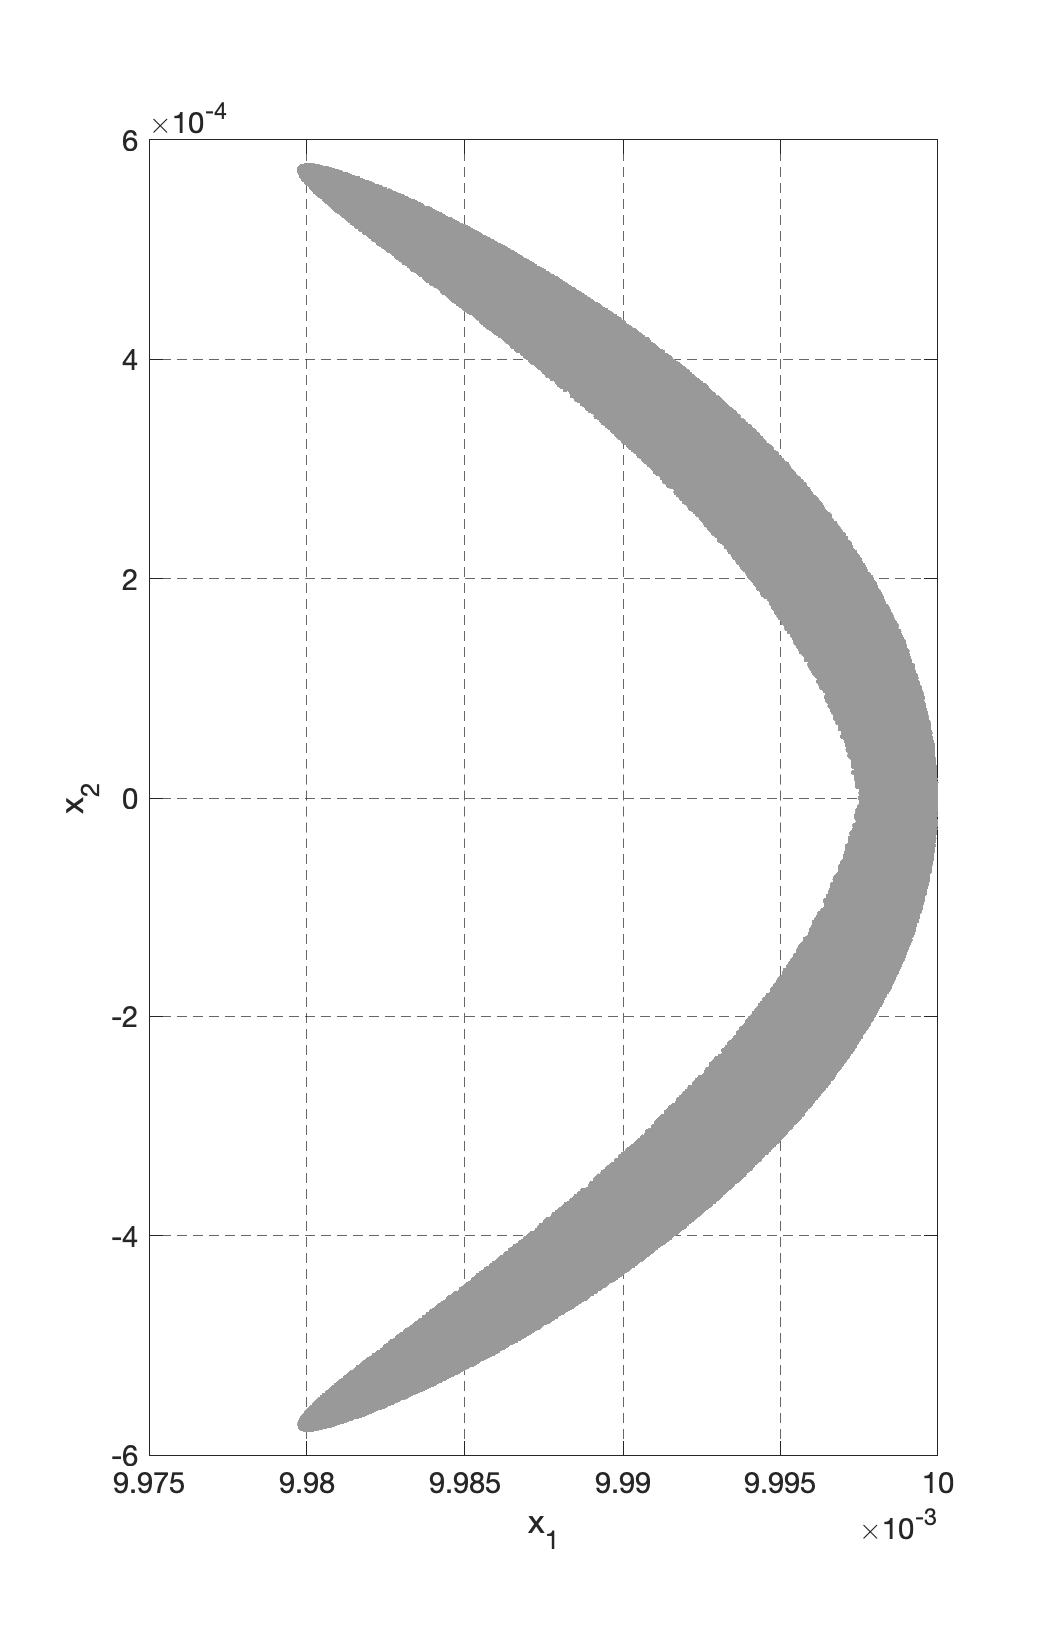
\includegraphics[width=\linewidth]{images/unicycle_u=0_x1-x2}
			\caption{$ G_{x_1,x_2}(\varepsilon) $}
			\label{fig:unicycleu0x1-x2}
		\end{figure}
		\column{0.32\textwidth}
		\begin{figure}
			\centering
			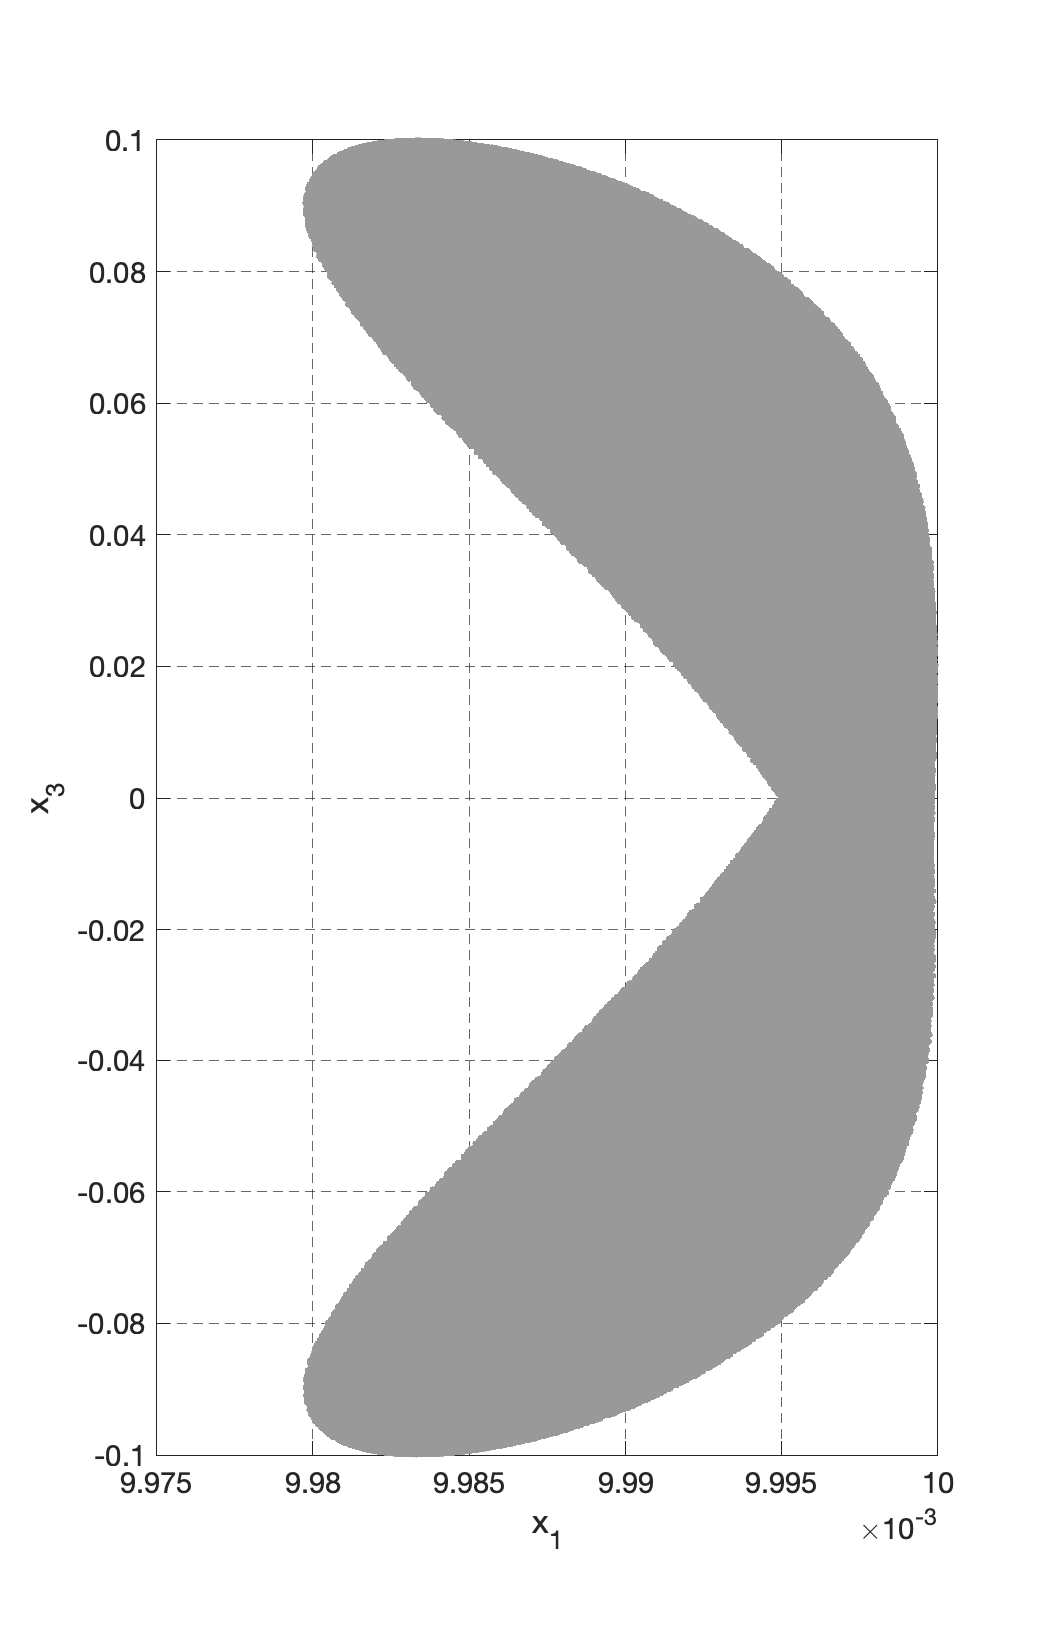
\includegraphics[width=\linewidth]{images/unicycle_u=0_x1-x3}
			\caption{$ G_{x_1,x_3}(\varepsilon) $}
			\label{fig:unicycleu0x1-x3}
		\end{figure}
		\column{0.32\textwidth}
		\begin{figure}
			\centering
			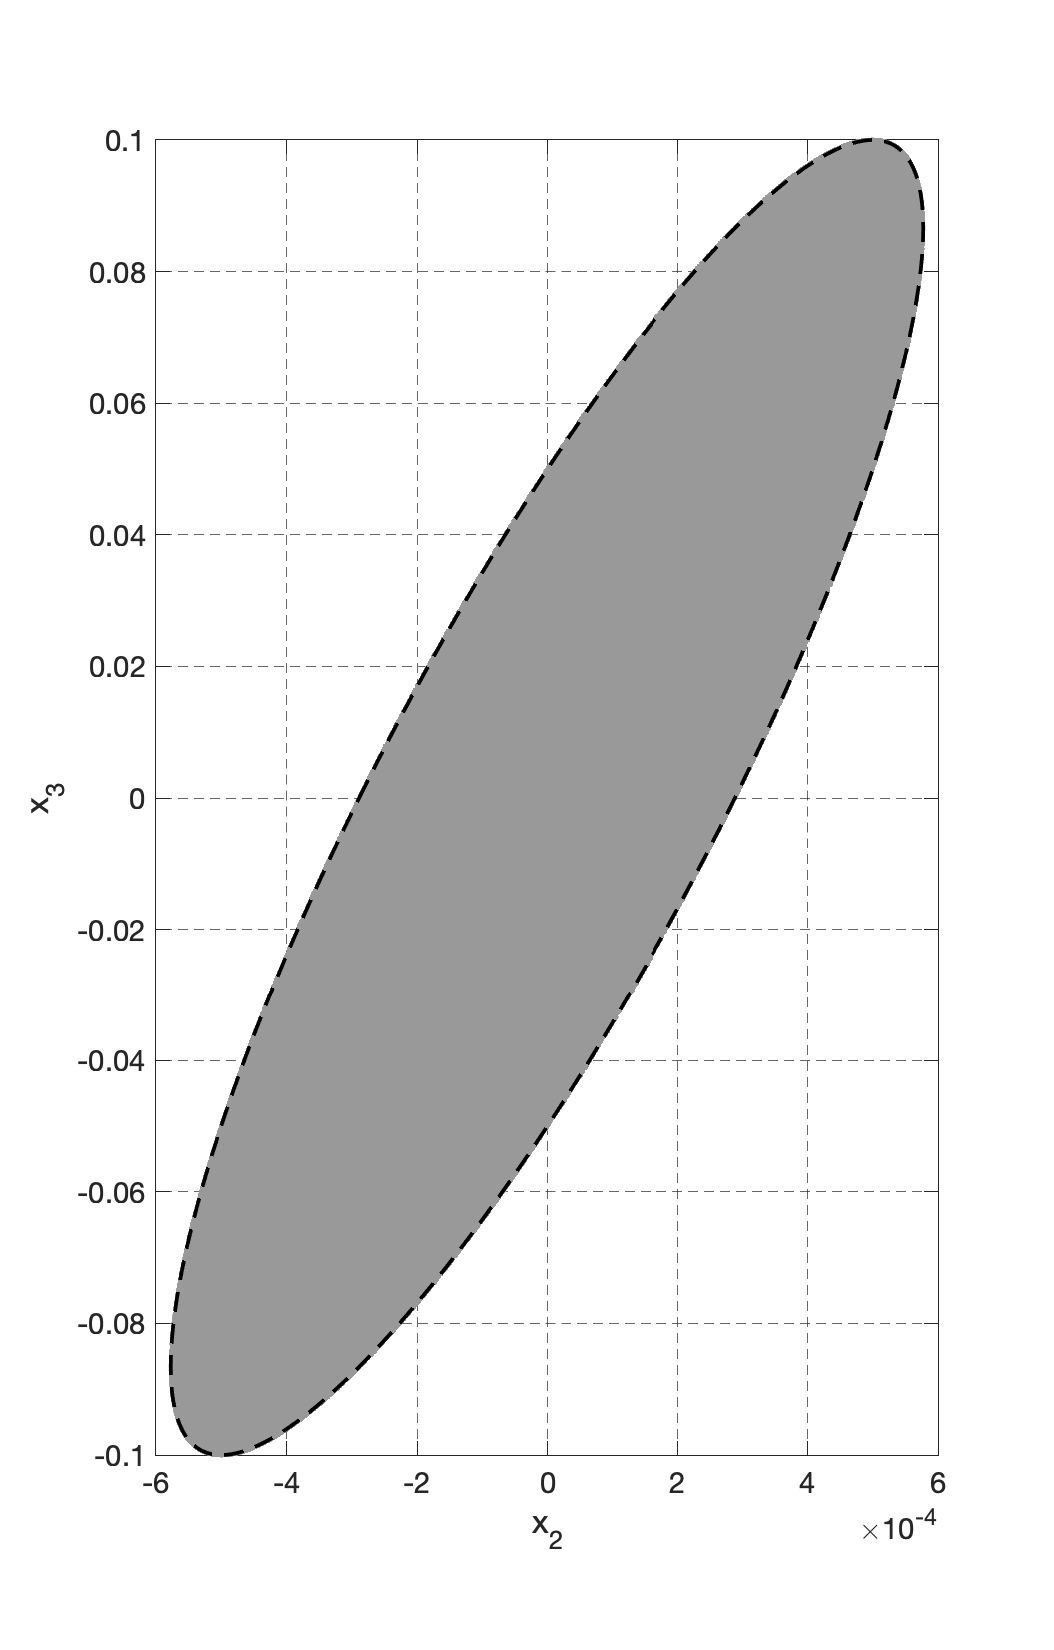
\includegraphics[width=\linewidth]{images/unicycle_u=0_x2-x3}
			\caption{$ G_{x_2,x_3}(\varepsilon) $}
			\label{fig:unicycleu0x2-x3}
		\end{figure}
	\end{columns}
\end{frame}


\begin{frame}
	\frametitle{Пример: Модифицированный уницикл}
	Рассмотрим систему
	\begin{equation}\label{unicycle1}
		\dot{x_1} = \cos(x_3), \qquad
		\dot{x_2} = \sin(x_3), \qquad
		\dot{x_3} = 1 + u(t), \qquad 0 \leqslant t \leqslant\varepsilon
	\end{equation}
	с ограничением на управление $ \displaystyle{\int_0^1} u^2(t) \, dt \leqslant 1 $. Это соответствует \eqref{unicycle0} с ограничением $ \displaystyle{\int_0^1} \left( u(t) - 1\right)^2 \ dt \leqslant 1 $.
	\begin{gather*}
		\widetilde{W}(\varepsilon) = \dfrac{1}{\varepsilon} W(\varepsilon) = 
	\end{gather*} \footnotesize
	\begin{gather*}
		=\begin{pmatrix} 
			\cos^2(\varepsilon)-\dfrac{3}{4\varepsilon}\sin(2\varepsilon)+\dfrac{1}{2} & 
			\cos\left(\varepsilon \right)\,\sin\left(\varepsilon \right)+\dfrac{1}{2\,\varepsilon}\left( 3\cos^2\left(\varepsilon \right)-2\cos\left(\varepsilon\right)-1\right) &
			\cos\left(\varepsilon \right)-\dfrac{1}{\varepsilon} \sin\left(\varepsilon \right) \\[8pt] 
			* &
			\dfrac{3}{2}-\dfrac{2\,\sin\left(\varepsilon \right)-\dfrac{3\,\cos\left(\varepsilon \right)\,\sin\left(\varepsilon \right)}{2}}{\varepsilon }-{\cos\left(\varepsilon \right)}^2 & \sin\left(\varepsilon \right)+\dfrac{1}{\varepsilon } \left(\cos\left(\varepsilon \right)-1 \right)\\
			* &
			* & 
			1 \end{pmatrix}.	
	\end{gather*}
	\normalsize
\end{frame}


\begin{frame}
	\frametitle{Пример: Модифицированный уницикл}
	\begin{enumerate} \footnotesize
		\item $ (x_1, x_2) $.  Условия Теоремы \ref{s2:th:assimptotic_equality} не выполняются.
		\begin{gather*}
			\widetilde{W}_{x_1,x_2}(\varepsilon) = \begin{pmatrix}
				\dfrac{2\,\varepsilon ^4}{15} + O(\varepsilon^6)&
				-\dfrac{5\,\varepsilon ^3}{24} + O(\varepsilon^5)\\[8pt]
				-\dfrac{5\,\varepsilon ^3}{24} + O(\varepsilon^5) & 
				\dfrac{\varepsilon ^2}{3}-\dfrac{3\,\varepsilon ^4}{20} + O(\varepsilon^6).
			\end{pmatrix}, \qquad \nu^{x_1,x_2}(\varepsilon) = \frac{1}{120}\varepsilon^4 + O(\varepsilon^6)
		\end{gather*}
		\item 	$ (x_1, x_3) $. Условия Теоремы \ref{s2:th:assimptotic_equality} не выполняются.
		\begin{gather*}
			\widetilde{W}_{x_1,x_3}(\varepsilon) = \begin{pmatrix} 
				\dfrac{2\,\varepsilon ^4}{15} + O(\varepsilon^6) &
				-\dfrac{\varepsilon^2}{3}+ O(\varepsilon ^4)\\[8pt]
				-\dfrac{\varepsilon^2}{3} + O(\varepsilon^4) & 1 \end{pmatrix}, \qquad  \nu^{x_1,x_3} =   \frac{1}{45}\varepsilon^4 + O(\varepsilon^6)
		\end{gather*}
		\item  $ (x_2, x_3) $. Условия Теоремы \ref{s2:th:assimptotic_equality} выполняются.  $ G_{x_2,x_3}(\varepsilon) $ выпукло и асимптотически эквивалентно соответствующему множеству линеаризованной системы.
		\begin{gather*}
			\widetilde{W}_{x_2,x_3}(\varepsilon)  = \begin{pmatrix}
				\dfrac{\varepsilon^2}{3} + O(\varepsilon^4) &
				\dfrac{\varepsilon }{2} + O(\varepsilon^3) \\[8pt]
				\dfrac{\varepsilon }{2} + O(\varepsilon^3) & 1
			\end{pmatrix}, \qquad \nu^{x_2,x_3}(\varepsilon) = \frac{\varepsilon^2}{12} + O(\varepsilon^4)
		\end{gather*}
	\end{enumerate}
\end{frame}


\begin{frame}
	\frametitle{Пример: Модифицированный уницикл}
	\begin{columns}
		\column{0.32\textwidth}
		\begin{figure}
			\centering
			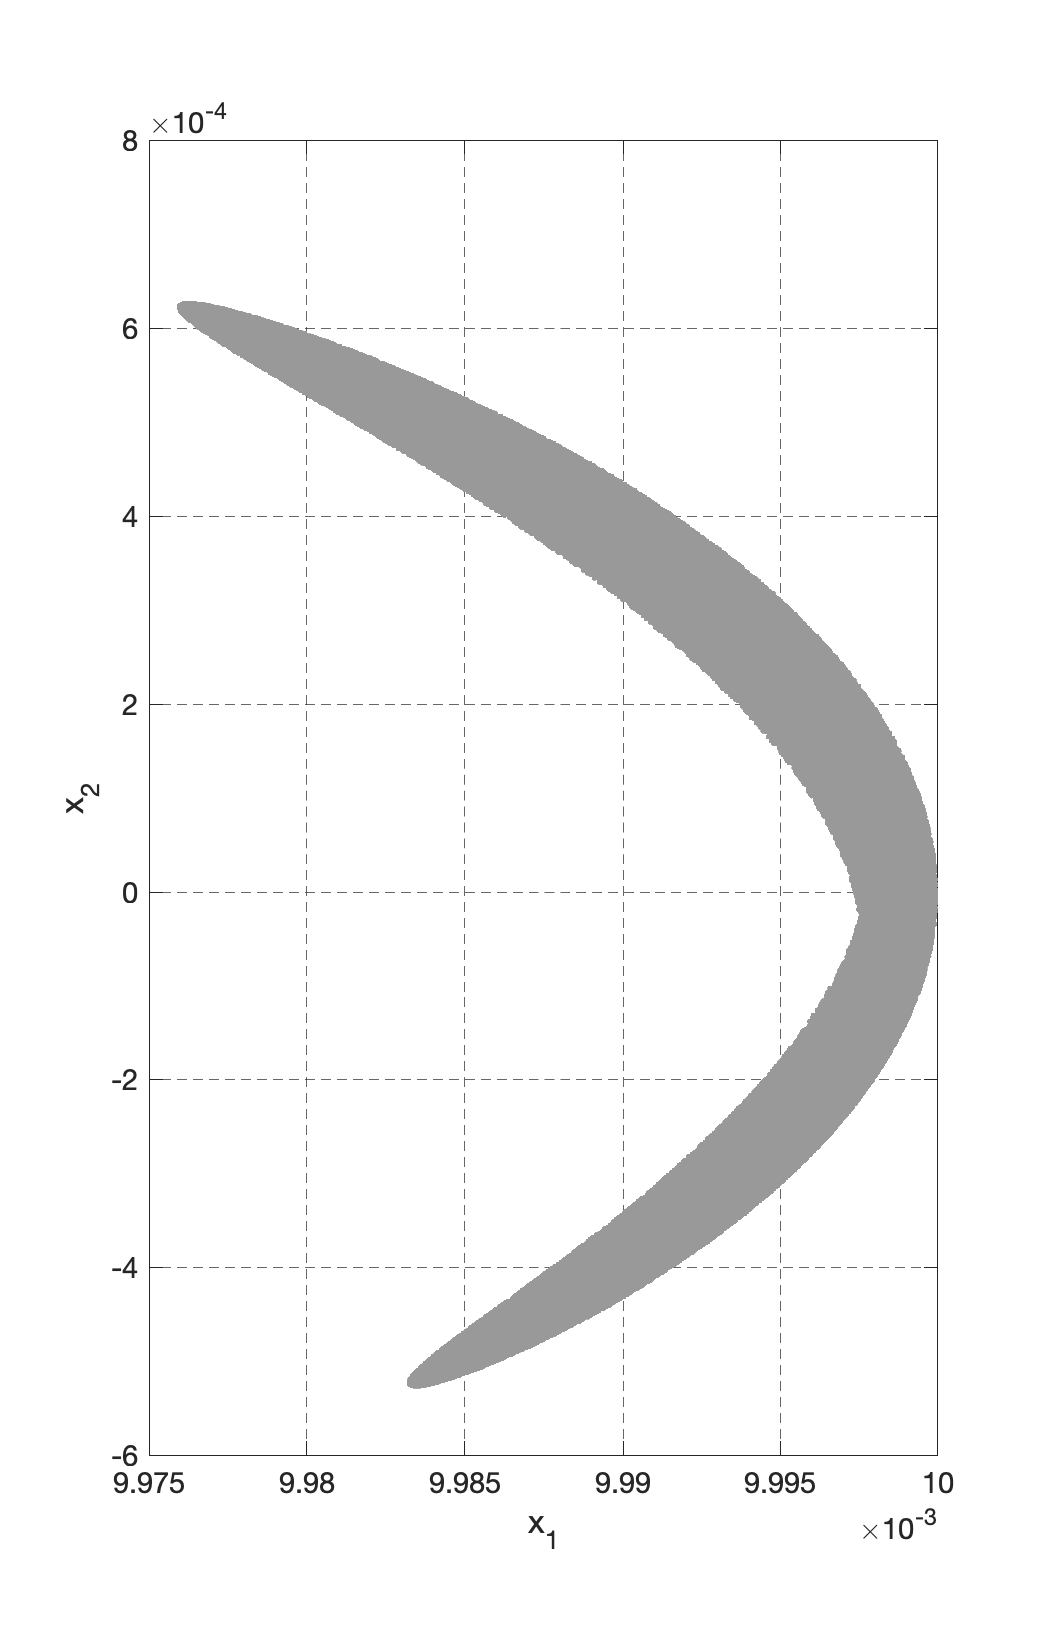
\includegraphics[width=\linewidth]{images/unicycle_u=1_x1-x2}
			\caption{$ G_{x_1,x_2}(\varepsilon) $}
			\label{fig:unicycleu1x1-x2}
		\end{figure}
		\column{0.32\textwidth}
		\begin{figure}
			\centering
			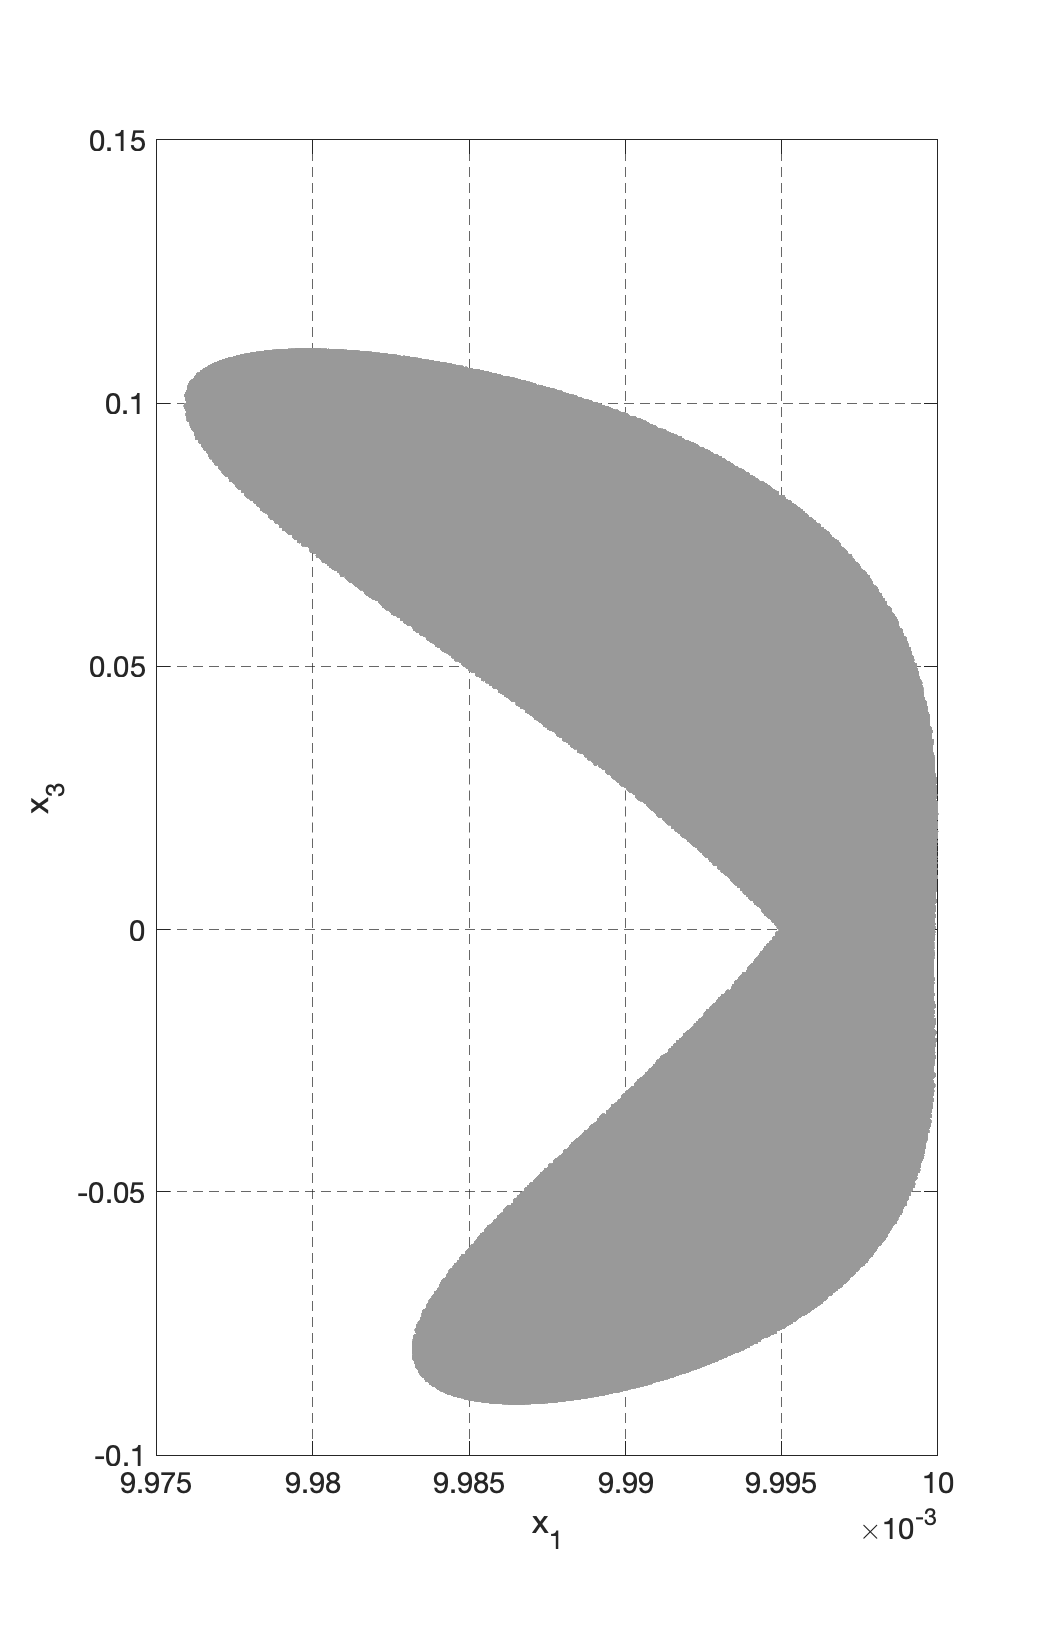
\includegraphics[width=\linewidth]{images/unicycle_u=1_x1-x3}
			\caption{$ G_{x_1,x_3}(\varepsilon) $}
			\label{fig:unicycleu1x1-x3}
		\end{figure}
		\column{0.32\textwidth}
		\begin{figure}
			\centering
			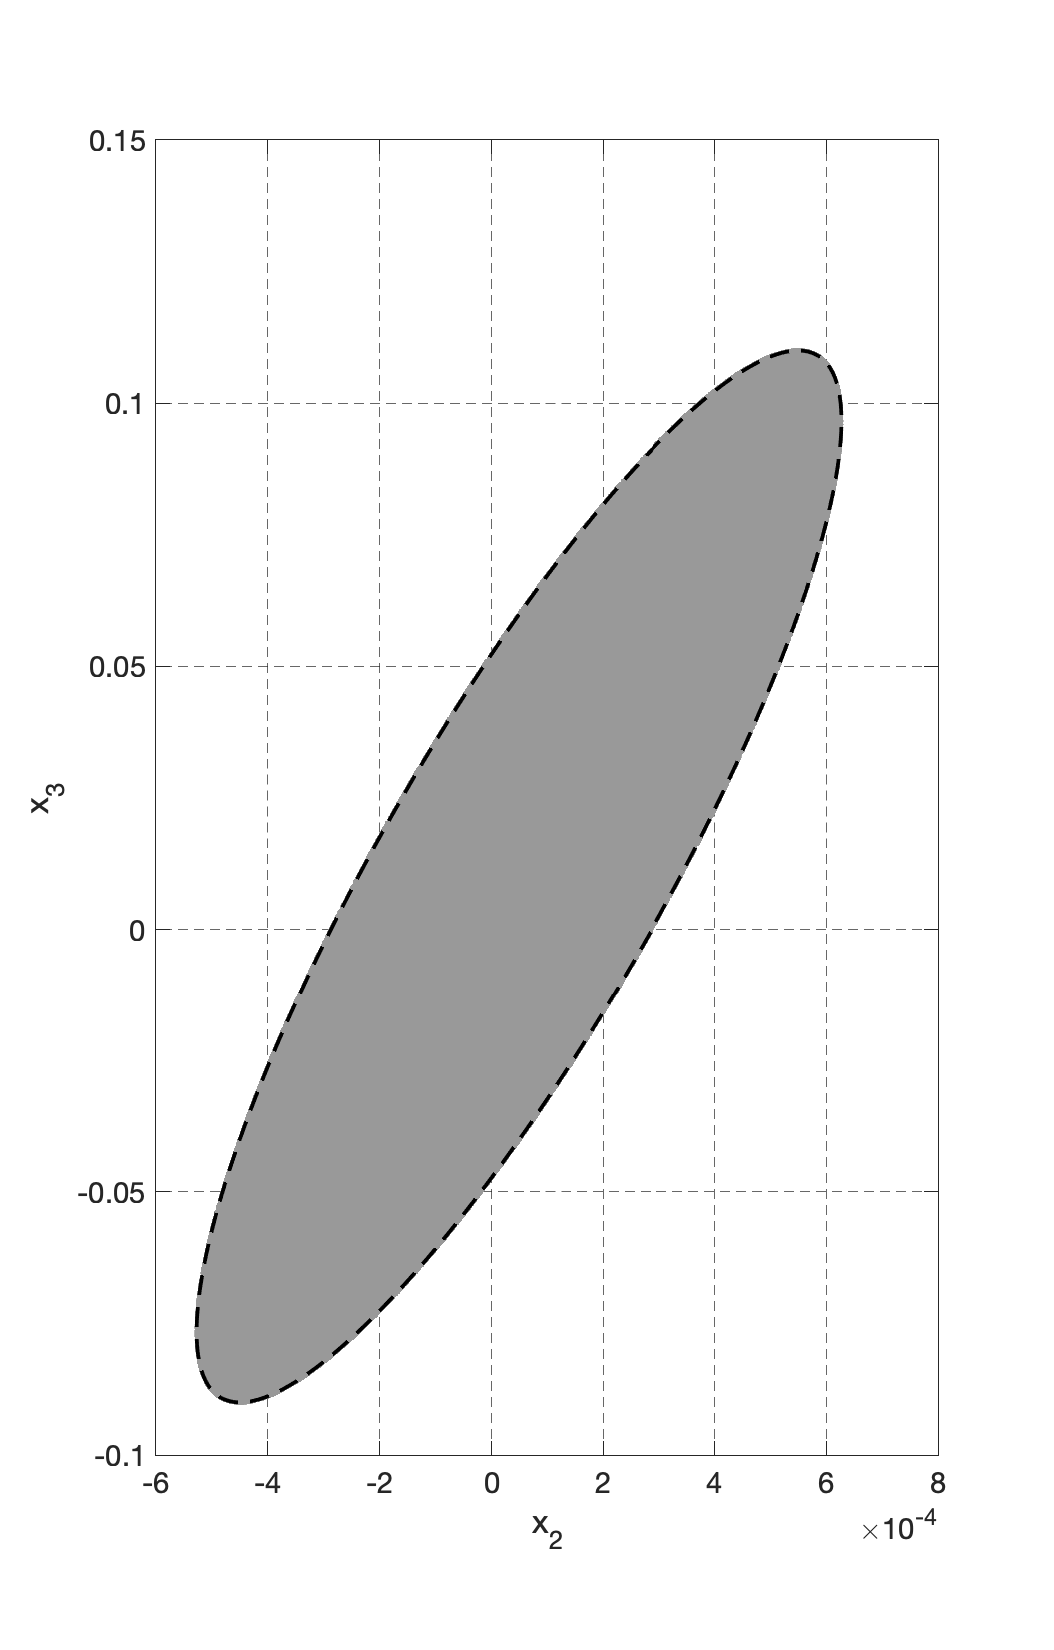
\includegraphics[width=\linewidth]{images/unicycle_u=1_x2-x3}
			\caption{$ G_{x_2,x_3}(\varepsilon) $}
			\label{fig:unicycleu1x2-x3}
		\end{figure}
	\end{columns}
\end{frame}

\begin{frame}{Условие применимости метода линеаризации в задаче локального синтеза}
Рассмотрим нелинейную систему, аффинную по управлению:
\begin{gather}\label{s22:nonlinear}
	\dot{z}(t)=f(z(t))+B u(t),\qquad 0 \leqslant t \leqslant T, \qquad z(0) = z_0,
\end{gather}
	\begin{asm}\label{s22:as:solution_bounded}
		Существует такое $\mu > 0$, что все решения $x(s, \upsilon(\cdot))$ системы \\ \mbox{$\dot{x} = -f(x)-B\upsilon(t)$}, выходящие из некоторой окрестности нуля и отвечающие управлениям $\upsilon(\cdot) \in B_{\mathbb{L}_2}(0, \mu)$, определены на интервале $[0, T]$ и лежат в шаре $ B_{\mathbb{R}^n}(0,\overline{r})$, $\overline{r} > 0$.
	\end{asm}
	\begin{asm}\label{s22:as:Residial_term_bounds}
		Найдутся такие $\overline{r} > r >0$, $k>0$, что при всех $ z \in B_{\mathbb{R}^n}(0,r) $ функция $f(z)$ может быть представлена в форме $ f(z) = Az + R(z) $, причём $A \in \mathbb{R}^{n \times n}$ и \mbox{$\|R(z) \| \leqslant k \| z\|^2$}. 
	\end{asm}
	Это свойство выполняется, если $f(0) = 0 $, $\frac{\partial f}{\partial z}(0) 
	= A $ и  функция $f(z)$ дважды непрерывно дифференцируема. 
\end{frame}

\begin{frame}{Постановка задачи синтеза}
		\begin{prb*}
		Синтезировать закон управления $u=u\big(t,z(t)\big)$, который бы приводил траектории замкнутой системы
		\begin{gather*}
			\dot{z}(t)=f(z(t))+B u(t,z(t)),\qquad 0 \leqslant t \leqslant T, \qquad z(0) = z_0
		\end{gather*}
		в начало координат в момент $T$ и обеспечивал при этом минимальное значение $I(T,u)=\int_0^Tu^\top (t)u(t)dt= \lVert u(\cdot)\rVert^2_{\mathbb{L}_2.}\to \min$. 
	\end{prb*}
\end{frame}

\begin{frame}{Линейный случай}
	Рассмотрим линейный случай ($R(z)=0$)
	\begin{gather}\label{s22:linear}
		\dot{z} = A z + B u, \qquad 0 \leqslant t \leqslant T.
	\end{gather}
	Если $(A,B)$ вполне управляема, то решение --- это линейный закон\footnote{\begin{itemize}\item
			Abgaryan K.A. Matrix Calculus with Applications in the Theory of Dynamical Systems Fizmatlit, Moscow, (1994)
			\item Kurzhanski, A.B., Varaiya, P.: Dynamics and Control of Trajectory Tubes. Theory and Computation. Birkhauser. (2014) \end{itemize}}
	\begin{gather}\label{s22:linear_feedback}
		u(t,z) = -B^{\top} Q_T(t) z, 
	\end{gather} где
	\begin{gather*}
		Q_T(t)=W^{-1}(T-t), \qquad W(t) = \int_0^t e^{-A\tau}BB^\top e^{-A^{\top}\tau}d\tau. 
	\end{gather*}
	\begin{ass}
		Любая траектория $z(t)$ системы \eqref{s22:linear} с управлением \eqref{s22:linear_feedback}, выходящая из точки $ z_0 $, достигает начала координат в момент $T$. 
		При этом интегральный функционал $I(T,u)$ принимает минимальное значение $z^{\top}_0 Q_T(0) z_0 $ при каждом $z_0$.
	\end{ass}
\end{frame}


\begin{frame}{Линейная обратная связь в нелинейном случае}
	Далее мы будем исследовать поведение траекторий системы \eqref{s22:nonlinear} замкнутой линейной обратной связью $ u(t,z) = -B^{\top} Q_T(t) z$
	\begin{equation}\label{nonlinear_closed}
		\dot{z} = f(z) - B B^{\top} Q_T(t) z, \qquad 0 \leqslant t \leqslant T, \qquad z(0) = z_0,
	\end{equation}
	где $Q_T(t)$ это решение уравнения
	\begin{gather*}
		\dot{Q}_T  = Q_T B B^{\top} Q_T - A^{\top}Q_T - Q_T A,\quad A = \frac{\partial f}{\partial x}(0), \quad Q_T(0) = W^{-1}(T).
	\end{gather*}
	 Известно, что при $T=\infty$ (задача стабилизации), линейная обратная связь, которая стабилизирует линейную систему, также будет стабилизировать и нелинейную систему в некоторой окрестности нуля.\\
	При каких условиях траектории \eqref{nonlinear_closed} будут стремиться к 0 (при достаточно малом $T$ )? \\
	Можно ли что-то сказать о значении интегрального функционала? 
\end{frame}

\begin{frame}{Система в обратном времени}
	Положив $\tau=T-t$, имеем
	\begin{gather}\label{s22:nonlinear_}
		\dot{x}(\tau)=-f(x(\tau))-B v(\tau),\qquad 0 \leqslant \tau \leqslant T,
	\end{gather}
	где $x(\tau)=z(T-\tau)$, $v(\tau)=u(T-\tau)$.
	
	множество достижимости системы \eqref{s22:nonlinear_}(или множество нуль-управляемости \eqref{s22:nonlinear})
	\begin{gather*}
		G_{-}(T,\mu)=\{x\in \mathbb{R}^n:\exists v(\cdot)\in B_{\mathbb{L}_2}(0,\mu),\; x=x\big(T,v(\cdot)\big)\}.
	\end{gather*} 
	Рассмотрим также линейную систему 
	\begin{gather}\label{s22:linear_}
		\dot{x}(\tau)=-Ax(\tau)-B v(\tau),\qquad 0 \leqslant \tau \leqslant T,
	\end{gather}
	Множество достижимости \eqref{s22:linear_} (или множество нуль-управляемости \eqref{s22:linear}) это эллипсоид \begin{gather*}
	 G_{-}^0(T,\mu)=\{x \in \mathbb{R}^n: x^\top W^{-1}(T)x\leqslant \mu^2\}
	\end{gather*}
\end{frame}

\begin{frame}{Функции $\varphi(\tau)$ и $\Phi(T)$}
	\begin{asm}\label{s22:asm1} 
		Пусть существуют $\overline{T}>0$ и непрерывная положительная функция $\varphi(\tau): (0, \overline{T}] \to \mathbb{R}$ такие, что
		\begin{gather*}
			0 < \frac{\eta(\tau)}{\sqrt{\nu(\tau)}} \leqslant \varphi(\tau), \qquad 0 < \tau \leqslant \overline{T},\quad \int\limits_0^ {\overline{T}}\varphi(\tau) d\tau<\infty.
		\end{gather*} 
		Здесь $\nu(\tau)$ и $\eta(\tau)$  --- это наименьшее и наибольшее собственные числа $W(\tau)$.
	\end{asm}
	Введём $\Phi(T)= \int\limits_0^ {T}\varphi(\tau) d\tau,\quad 0 <  T \leqslant \overline{T},\quad  \Phi(0)=0. $ 
	\begin{itemize}
		\item[\emoji{one}] Если $\Phi(T) < \infty $ хотя бы для одного $T$, то $\Phi(T) < \infty $ для всех $T \in (0, \overline{T})$.
		\item[\emoji{two}] $\Phi(T) \in  C^1(0,\overline{T})$.
		\item[\emoji{three}] $\Phi(T) $ возрастает.
	\end{itemize}
	\begin{asm}\label{s22:asm2}
		Существует такое $ 0 < \beta \leqslant 1$, что $\frac{\sqrt{\eta(T)}}{\Phi^\beta(T)} \to 0$ при $T \to 0$.
	\end{asm}
\end{frame}

\begin{frame}{Оценки для квадратичной формы}
	Обозначим $ V_T(t,z) = z^{\top}(t)Q_T(t)z(t)$, где $z(t)$ --- это решение \eqref{nonlinear_closed}.
	Продифференцируем $V_T$
	\begin{gather}\label{dvt_first}
		\begin{gathered}
			\frac{d}{dt}V_T = \frac{d}{dt}z^{\top}(t)Q_T(t)z(t) = 2 \langle R(z), Qz\rangle - z^{\top} Q B B^{\top} Q z \leqslant \\ \leqslant 
			2 \langle R(z), Qz\rangle \leqslant 2 \| R(z) \|_{Q_T} \| z \|_{Q_T} = 2 \| R(z) \|_{Q_T} V_T^{\frc{1}{2}}.
		\end{gathered}
	\end{gather}
	\begin{lem}\label{s22:lem:vest}
		Пусть выполнено предположение \ref{s22:asm1}. 
		Если $T\leqslant \check{T}$ и $z(t)$ --- такая траектория системы \eqref{nonlinear_closed}, что $z(t) \in B(0,r)$ при $0<t \leqslant T$ и $V_T(0,z(0))\leqslant 1/(4k^2\Phi^{2\beta}(T))$ для некоторого $0<\beta \leqslant 1$, то
		\begin{gather*}
			V_T(t,z(t)) \leqslant \frac{1}{k^2\Phi^{2\beta}(T)}, \qquad 0 \leqslant t \leqslant T. 
		\end{gather*}
	\end{lem}
	\emoji{arrow-down-small} Доказывается при помощи теоремы сравнения и  \eqref{dvt_first}.
\end{frame}


\begin{frame}{Асимптотика замкнутой системы}
	\begin{thm}\label{s22:th:tends_to_zero}
		Пусть выполнены предположения \ref{s22:asm1}, \ref{s22:asm2}. 
		Тогда существует момент $ T_1 \leqslant \check{T}$, что для всех $ T \leqslant T_1$ найдётся такое $ r_1(T)$, что траектории системы \eqref{nonlinear_closed}, выходящие из $z(0) = z_0 \in B(0,r_1(T))$, стремятся к $0$ при $t \to T$.
	\end{thm}
	\begin{itemize}
		\item[\emoji{arrow-down-small}\emoji{one}] Так как $\frac{\sqrt{\eta(T)}}{\Phi^\beta(T)} \to 0$, $\exists T_2 \leqslant T_1$, что $\frac{\sqrt{\eta(T)}}{k\Phi^\beta(T)}  \leqslant \frac{r}{2}$, $0 < T \leqslant T_2$.
		\item[\emoji{two}] Выберем $r_1(T) = \min \left\{ \frac{r}{4}, \frac{\sqrt{\nu(T)}}{2k\Phi^\beta(T)} \right\}$.
		\item[\emoji{three}] Используя Лемму  \ref{s22:lem:vest} можно доказать, что $z(t) \in B(0,r) $. 
		\item[\emoji{four}] Тогда, $ \|z(t)\|^2 \leqslant \eta(T-t)\psi(t) \leqslant \eta(T-t)\big(k^2\Phi^{2\beta}(T)\big)^{-1} $,\\
		где $\eta(T-t) \to 0$ при $t \to T$, что означает, что $\|z(t)\|$ тоже стремится к нулю. \emoji{chequered-flag}
	\end{itemize}
	% Role of beta
\end{frame}

\begin{frame}{Связь Теорем \ref{s22:th:tends_to_zero} и \ref{s2:th:assimptotic_equality}}
	\begin{cor}%\label{cor:1}
	Пусть существуют такие $ l > 0$, $\tau_0 > 0$ и $\alpha > 0$, что для всех $0 < \tau \leqslant \tau_0 $ выполняется неравенство
	\begin{gather}\label{s22:asymp}
		\nu(\tau)\geqslant l\tau^{4-\alpha}.
	\end{gather}
	Тогда справедливы Предположения \ref{s22:asm1} и \ref{s22:asm2} и, следовательно, утверждение Теоремы \ref{s22:th:tends_to_zero} является верным.
	\end{cor}
	\begin{itemize}
		\item[\emoji{arrow-down-small}\emoji{one}] Положим $\overline{T}=\tau_0$.
		\item[\emoji{two}] $\exists \tau>0$, такое, что $\eta(\tau)  \leqslant m\tau $
		\item[\emoji{three}] Имеем $\eta(\tau)/\sqrt{\nu(\tau)} \leqslant  ml^{-1/2}\tau^{-1+\alpha/2},$ и можем выбрать  $\varphi(\tau):= ml^{-1/2}\tau^{-1+\alpha/2}$
		\item[\emoji{four}] В этом случае $\Phi(T)=2mT^{\alpha/2}/(l^{-1/2}\alpha)$, и Предположения \ref{s22:asm1} выполняется.
		\item[\emoji{five}] Так как $\sqrt{\eta(T)}/\Phi^\beta(T) \leqslant c_0T^{(1-\alpha\beta)/2},$ где $c_0$ --- константа, то для выполнения Предположения \ref{s22:asm2}, достаточно выбрать $\beta < 1/\alpha$.  \emoji{chequered-flag}
	\end{itemize}
\end{frame}

\begin{frame}{Оценка погрешностей в значениях функционала}
	Проинтегрируем \eqref{dvt_first} от $0$ до $t$:
	\begin{gather}\label{s22:J}
		z^{\top}(t) Q_T(t)z(t) = z_0^{\top} Q_T(0)z_0 - \int_{0}^{t} u^{\top}(\xi) u(\xi) \, d\xi + 2\int_{0}^{t} R^{\top}(z(\xi))Q_T(\xi) z(\xi) d\xi,
	\end{gather}
	 где $ u(\xi) = -B^{\top} Q_T(\xi) z(\xi)$ --- управление в момент времени $\xi$.  \\
	\emoji{check-mark}В линейном случае, $R(z) \equiv 0$ и $z^{\top}(t) Q_T(t)z(t) \to 0 $ при $t \to T$
\begin{gather*}
	J_0(T,z_0) = z_0^{\top} Q_T(0)z_0 = \int_{0}^{t} u^{\top}(\xi) u(\xi) \, d\xi.
\end{gather*}
	В нелинейном случае возникает два вопроса: \\
	$z^{\top}(t) Q(t)z(t) \to 0$? \\
	Что можно сказать о
	\begin{gather*}%\label{gamma}
		\gamma (t,z_0) = 
		2\int_{0}^{t}  R^{\top}\big(z(\xi,z_0)\big)Q(\xi) z(\xi,z_0) d\xi?
	\end{gather*}
\end{frame}

\begin{frame}{Оценка погрешности функционала}
	\begin{thm}\label{s22:th:functional_error_estimate}
		Пусть выполнено предположение \ref{s22:asm1}. 
		Пусть $x(t)$ --- такая траектория системы \eqref{nonlinear_closed}, что $x(t)\in B(0,r)$ при $0\leqslant t \leqslant \tilde{T} \leqslant \overline{T} $ и $V_{\tilde{T}}(t,x(t))\to 0$ при $t\to \tilde{T}$. 
		Тогда существует такое $T_2 \leqslant \tilde{T}$, что для всех $0 < T < T_2 $ выполняется следующая оценка:
		\begin{gather} \label{s22:est}
			\left| \frac{ J(T) - J_0(T)}{J_0(T)}\right| \leqslant 16k\Phi({T})J^{1/2}_0(T).
		\end{gather}
		Здесь $J(T)=J(T,x(\tilde{T}-T))$, $J_0(T)=J_0(T,x(\tilde{T}-T))$ --- значения функционала $I(T,u(\cdot))$ на траекториях нелинейной и линеаризованной систем соответственно.
	\end{thm}
	\emoji{arrow-down-small}\emoji{one} Пусть $T\leqslant \tilde{T}$, $\tau=\tilde{T}-T+t$ и $z(t)$ --- траектория \eqref{nonlinear_closed} при $z(0)=x(\tilde{T}-T)$ при $[0,T)$.  Тогда имеем
	\begin{gather*}
		V_T(t,z(t))=z^\top(t)Q_T(t)z(t)=V_{\tilde{T}}(\tau,x(\tau)), \\
		V_T(0,z(0))=V_{\tilde{T}}(\tilde{T}-T, x(\tilde{T}-T)),
	\end{gather*}
	Так как  $V_{\tilde{T}}(t,x(t))\to 0$,  $t\to \tilde{T}$ получаем $V_T(0,z(0))=J_0(T) \to 0 $, $T\to 0$.
\end{frame}


\begin{frame}{Оценка погрешности функционала}
	\emoji{two} Перепишем \eqref{s22:J} 
	\begin{gather*}
		\underbrace{\int_{0}^{T} u^{\top}(\xi)  u(\xi) \, d\xi}_{J(T)} - \underbrace{z_0^{\top} Q_T(0)z_0}_{J_0(T)}= 2\int_{0}^{T}  R^{\top}(z(\xi))Q(\xi) z(\xi) d\xi=\gamma(T,z(0)),
	\end{gather*}
	\emoji{three} Из Леммы \ref{s22:lem:vest} следует, что
	\begin{gather*}
		\gamma (T,z(0)) = 
		2\int_{0}^{T}  R^{\top}(z(\xi))Q_T(\xi) z(\xi) d\xi\leqslant 2k \Phi(T) (4J_0(T))^{3/2}  
	\end{gather*}
	\emoji{chequered-flag}
\end{frame}

\begin{frame}{Стремление $z^{\top}(t) Q(t)z(t) $ к нулю}
	\begin{thm}
		 Пусть выполнено неравенство \eqref{s22:asymp}. 
		Пусть $T \leqslant \overline{T}$ и траектория $z(t)$ системы \eqref{nonlinear_closed} стремится к нулю при $t\to T$. 
		Тогда $V_{T}(t,z(t)) =z^{\top}(t)Q_T(t)z(t) \to 0$ при $t \to T$.
	\end{thm}
	\begin{itemize}
		\item[\emoji{arrow-down-small}\emoji{one}] $ u(\xi) = -B^{\top} Q(\xi) z(\xi)$ непрерывно при $0 \leqslant \xi <T$.
		\item[\emoji{two}] Из \eqref{s22:asymp} следует, что $V_{T}(t,z(t))$ ограничена и  $I(t,u) = \int_{0}^{t} u^{\top}(\xi)u(\xi) d\xi$  равномерна ограничена на  $t\in [0,T]$
		\item[\emoji{three}] Из асимптотической эквивалентности $G_{-}^0$, $ G_{-}$ и  свойств расстояния Банаха-Мазура следует \begin{gather*}
			V_{T}(t,z(t)) =z^{\top}(t)Q(t)z(t) \to 0  \mbox{ as } t \to T.
		\end{gather*}
	\end{itemize}
\end{frame}

\begin{frame}{Пример. Осциллятор Дуффинга}
	Рассмотрим двухмерную нелинейную систему
	\begin{gather}\label{Duffing}
		\dot{z}_1 = z_2, \quad \dot{z}_2 = -z_1 - 10z_1^3 + u, \quad 0\leqslant t 
		\leqslant T
	\end{gather}
	Желаемое конечное состояние $ x_1(T) = x_2(T) =  0 $.
	Матрицы линеаризованной в 0 системы:
	\begin{gather}\label{LinearDuffing}
		A = \begin{pmatrix} 0 & 1\\
			-1 & 0
		\end{pmatrix}, \quad B = \begin{pmatrix}
			0\\
			1
		\end{pmatrix}.
	\end{gather}
	\emoji{check-mark-button} Предположение \ref{s22:as:Residial_term_bounds} выполняется при $k = 10$, $r = 1$: 
	\begin{gather*}
		\|R(z)\| = 10|z_1|^3 < 10 (z_1^2+z_2^2), \qquad z_1^2+z_2^2 \leqslant 1
	\end{gather*}
	\emoji{check-mark-button} Условия Теоремы \ref{s22:th:tends_to_zero} тоже выполнены, 
	\begin{gather*}
		\nu(t) = \frac{t^3}{12} + O(t^5), \qquad \eta(t) = t - \frac{t^3}{12}+ O(t^5), \qquad  \varphi(t) = \frac{4}{\sqrt{t}}, \\
		\Phi(T) = 8\sqrt{T}, \quad \beta = 0.25, \quad \frac{\sqrt{\eta(T)}}{\Phi^\beta(T)} =  t^{0.25}\sqrt{0.125t^4-2.5t^2+30}
	\end{gather*}
\end{frame}

\begin{frame}
	\frametitle{Пример. Осциллятор Дуффинга}
	\begin{figure}
		\centering
		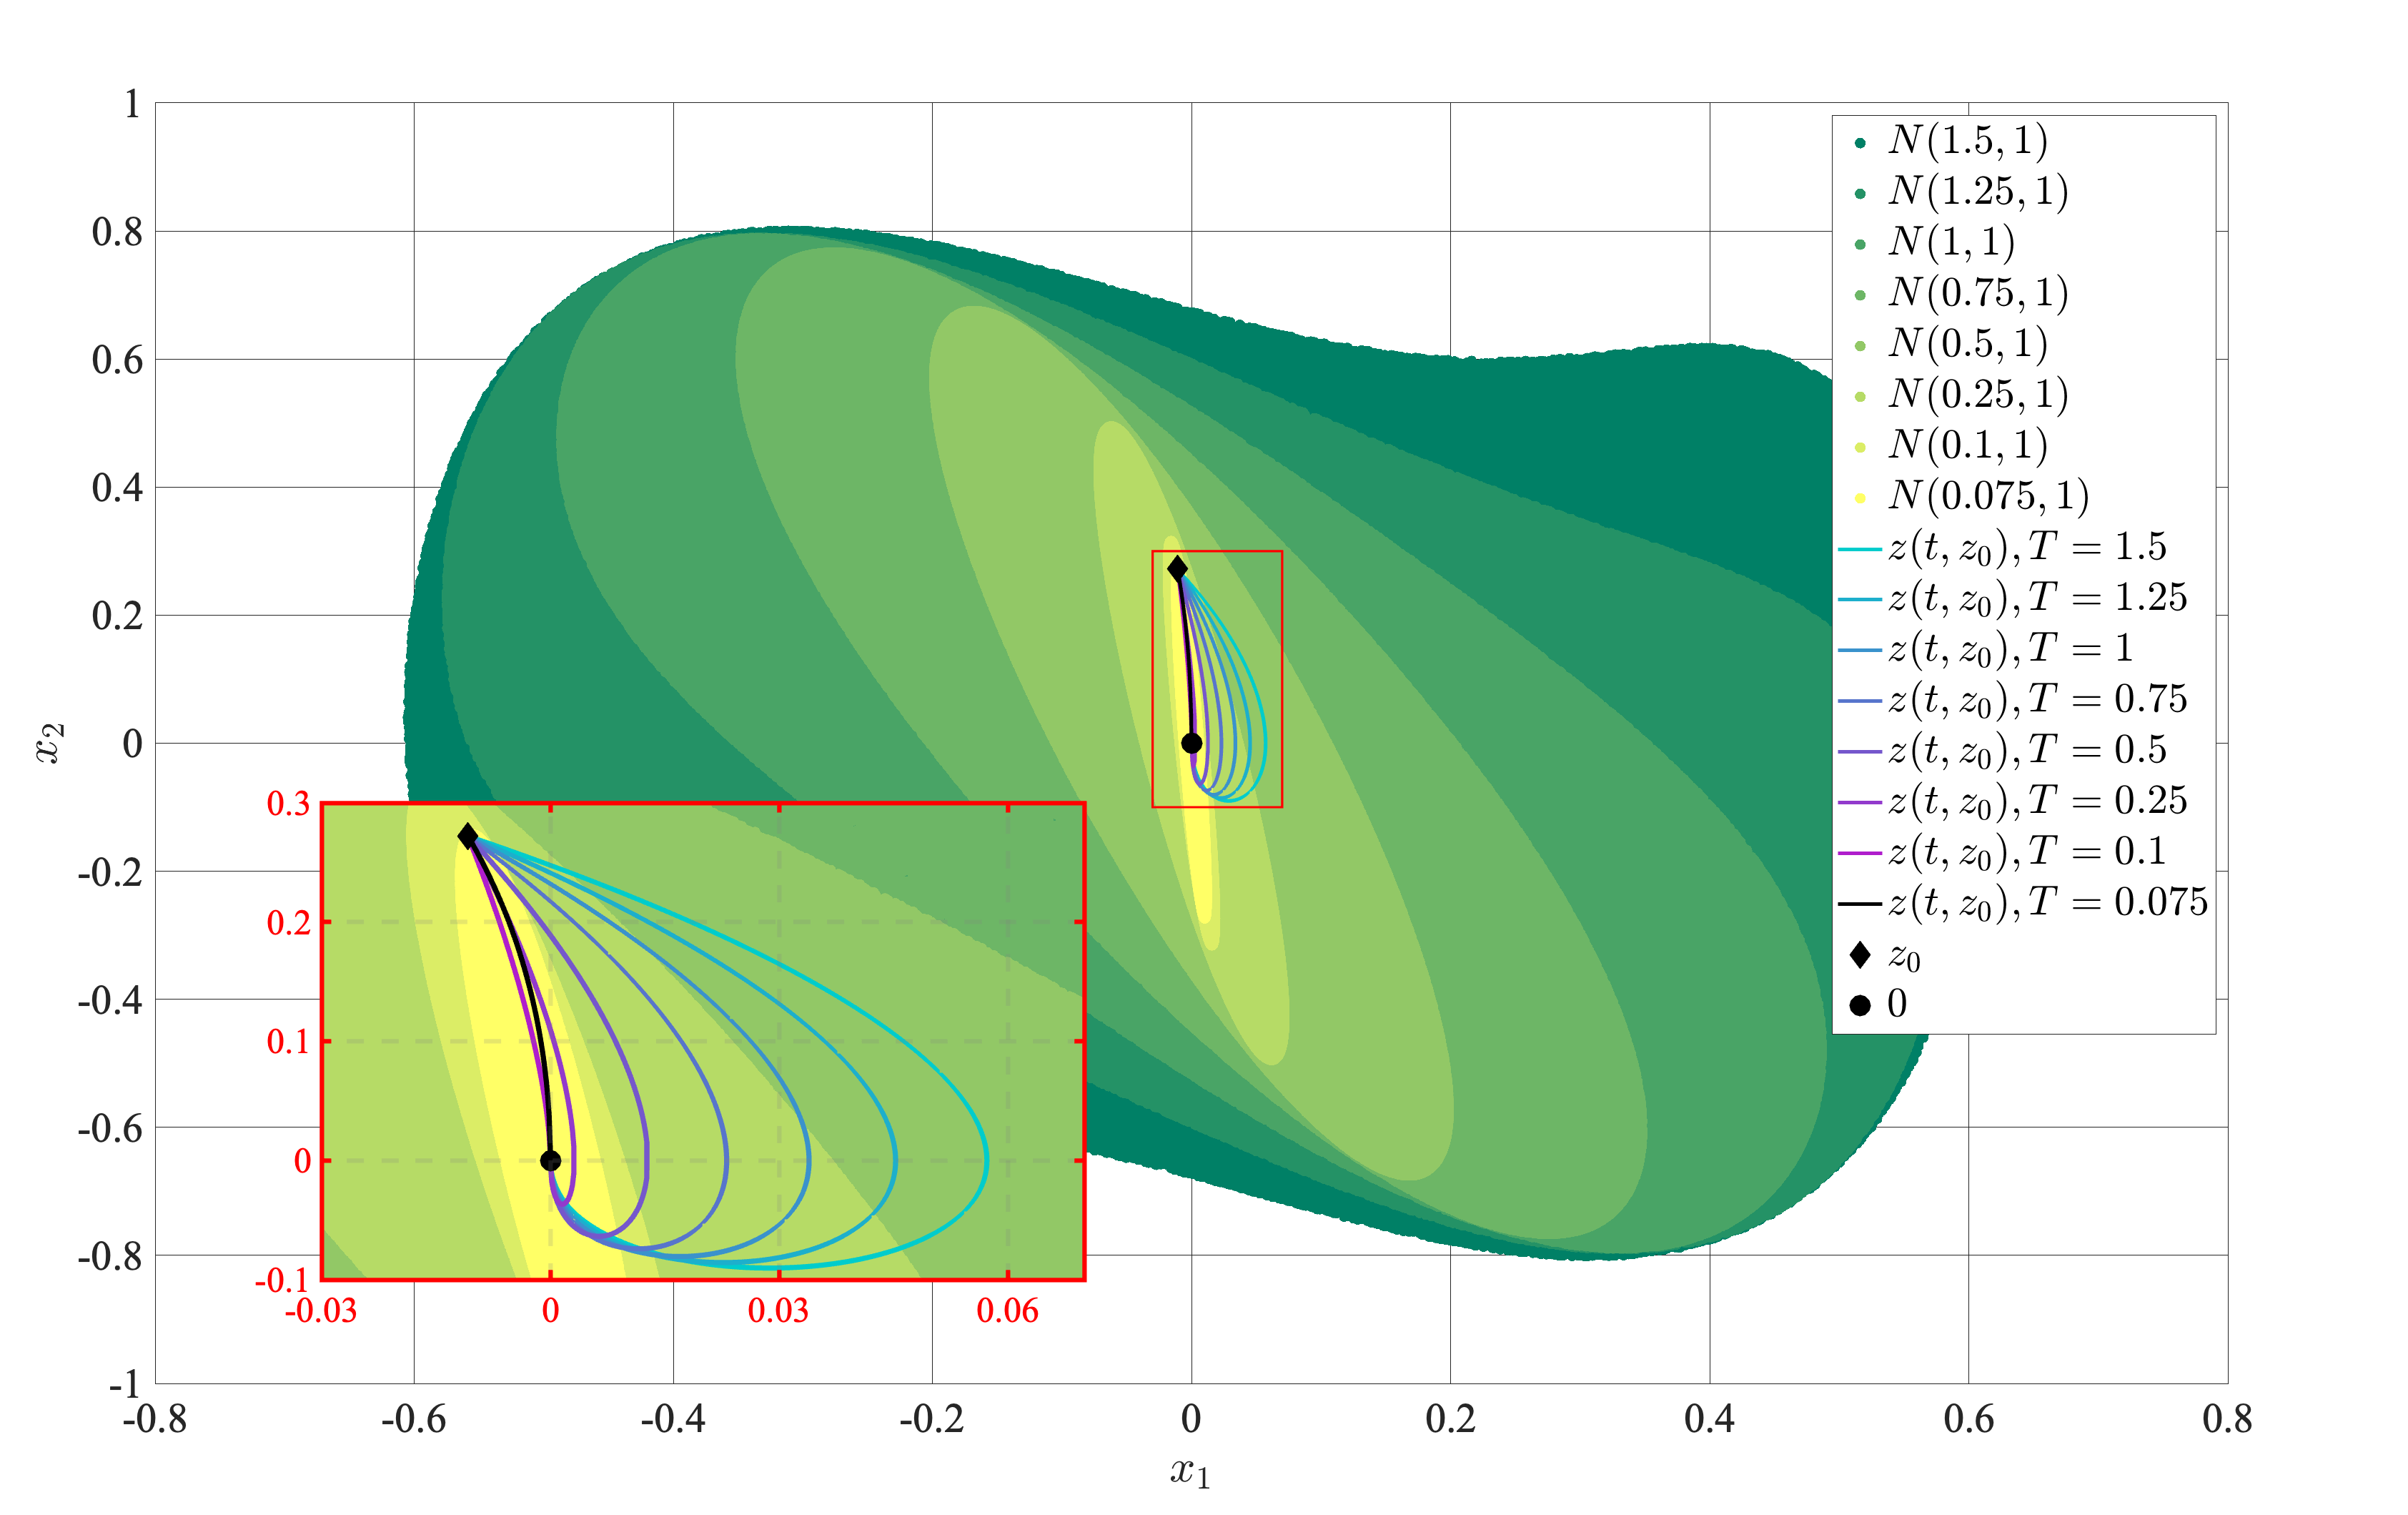
\includegraphics[width=0.9\linewidth]{images/GusevMIOsipov_Duffing_fixed_z0}
	\end{figure}
\end{frame}

\begin{frame}{Пример. Осциллятор Дуффинга}
	\begin{table}
		\label{ExampleTable1}
		\begin{center}
			\begin{tabular}{c|c|c|c|c}
				№ & $T$   &  $z_0^{\top} Q_T(0) z_0$   & $ J(T,z_0) $  & $ 
				\gamma (t,z_0) $   \\ \hline 
				1 & 1.500 & 0.159686  & 0.159136 & 0.0034435   \\ \hline
				2 & 1.250 & 0.197308  & 0.197031 & 0.0013990   \\ \hline
				3 & 1.000 & 0.249346  & 0.249231 & 0.0004611  \\ \hline
				4 & 0.750 & 0.327395  & 0.327360 & 0.0001055   \\ \hline
				5 & 0.500 & 0.459094 & 0.459089 & 0.0000102   \\ \hline
				6 & 0.250 & 0.710789  & 0.710790 & 0.0000012   \\ \hline
				7 & 0.100 & 0.836541  & 0.836542 & 0.0000014   \\ \hline
				8 & 0.075 & 1.000000  & 1.000001 & 0.0000009   \\ \hline
			\end{tabular}
		\end{center}
	\end{table} 
\end{frame}

\begin{frame}{Пример. Осциллятор Дуффинга}
	\begin{figure}
		\centering
		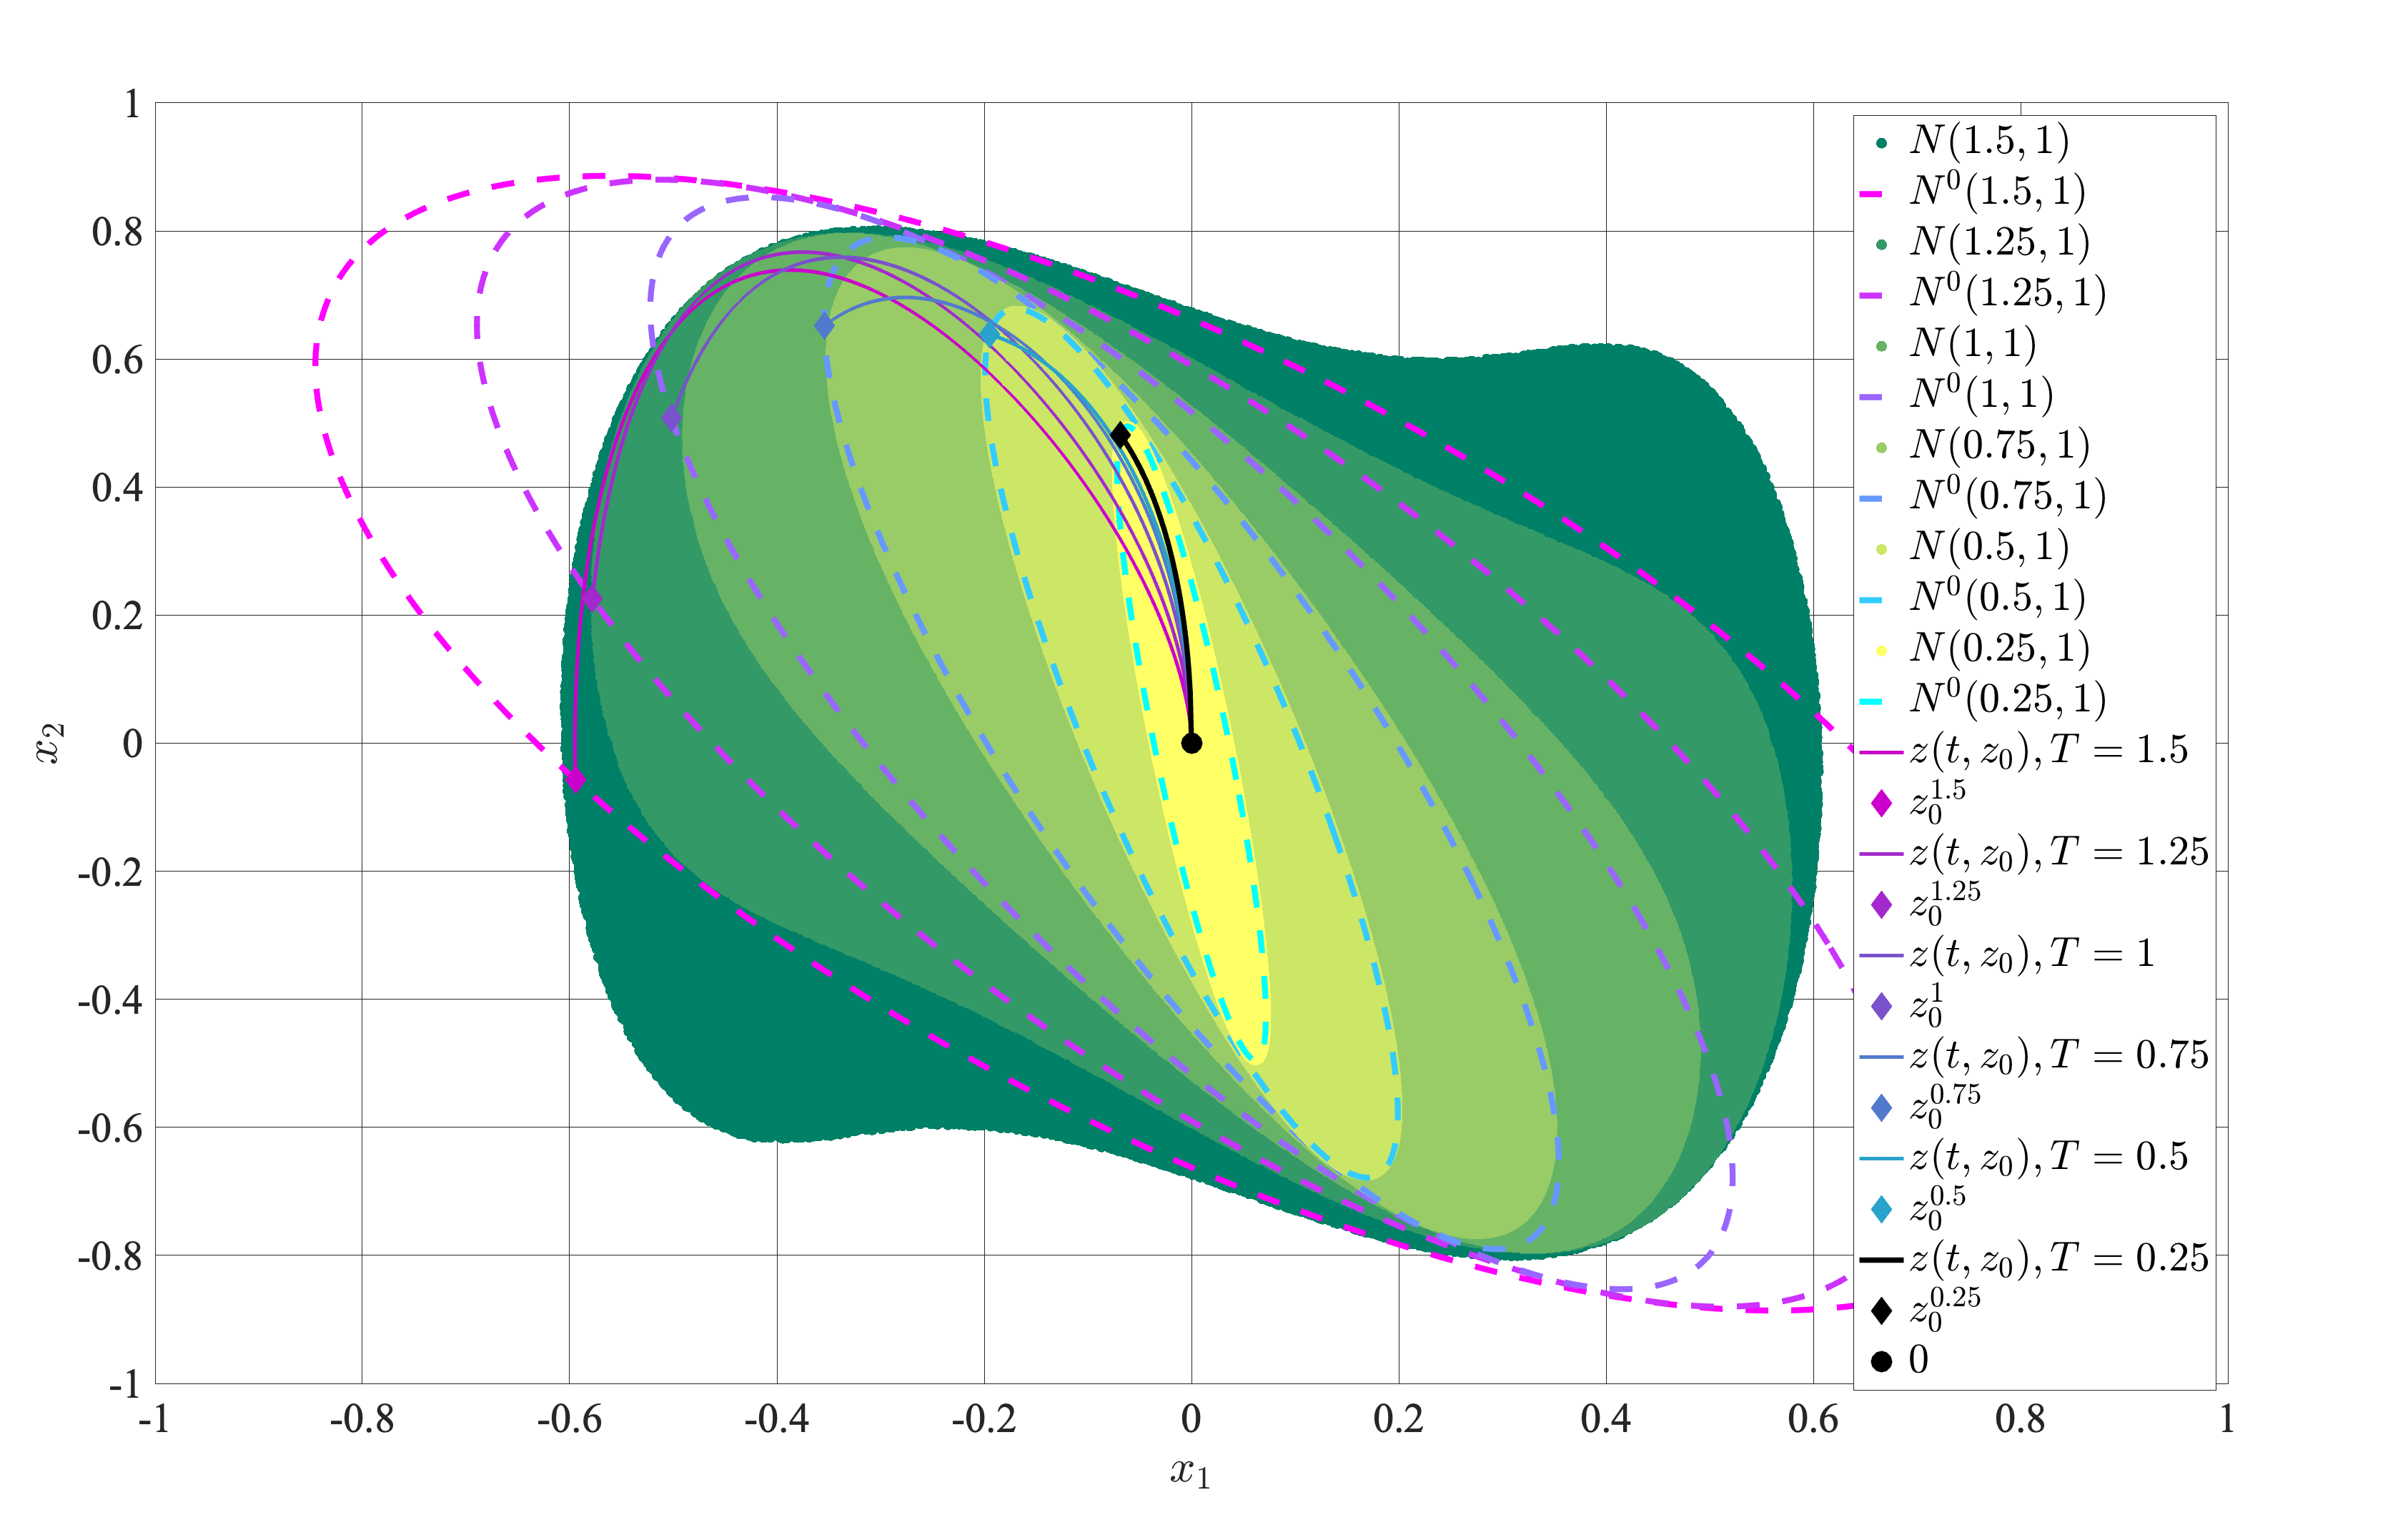
\includegraphics[width=0.9\linewidth]{images/GusevMIOsipov_Duffing_variable_z0}
	\end{figure}
\end{frame}

\begin{frame}{Пример. Осциллятор Дуффинга}
	\begin{table}
		\label{ExampleTable2}
		\begin{center}
			\begin{tabular}{c|c|c|c|c|c}
				$T$  & $z_0$            & $\|z_0\|^2$&$z_0^{\top} Q_T(0) z_0$ &$J(T,z_0)$&$\gamma (t,z_0)$ \\ \hline 
				1.500 & [-0.594;-0.057]  & 0.356680   & 0.999993    & 1.075833 & 0.0758407 \\ \hline
				1.250 & [-0.578;0.226]   & 0.385032   & 0.999997    & 1.110464 & 0.1104671 \\ \hline
				1.000 & [-0.502;0.508]   & 0.509514   & 0.999999    & 1.108159 & 0.1081607 \\ \hline
				0.750 & [-0.354;0.652]   & 0.550391   & 1.000000    & 1.048784 & 0.0487844 \\ \hline
				0.500 & [-0.195;0.638]   & 0.445513   & 1.000000    & 1.009848 & 0.0098475 \\ \hline
				0.250 & [-0.069;0.481]   & 0.236487   & 1.000000    & 1.000349 & 0.0003490 \\ \hline
			\end{tabular}
		\end{center}
	\end{table} 
\end{frame}

\section{Глава 3}
	
	\begin{frame}{Глава 3. Выпуклость множеств достижимости}
		Была исследована выпуклость множеств достижимости в следующих постановках
		\begin{itemize}
			\item[\emoji{one}] 
			Нелинейная аффинная по управлению система с малым ресурсом управления\footnote{Polyak~B.\,T. Convexity of the reachable set of nonlinear systems under L2 bounded controls~// Dynam. Contin. Discrete Impuls. Systems Ser. A Math. Anal. --- 2004. --- Vol.~11, Suppl.~2-3. --- P.~255--267}.
			\begin{gather*}
				\dot{x}(t) = f_1(t,x(t)) + f_2(t,x(t)) u(t), \quad t_0 \leqslant t \leqslant T, \quad x(t_0) = x_0, \\
				u(\cdot) \in \left\{u(\cdot) \in \mathbb{L}_2: \int\limits_0^T u^{\top}(t)u(t) dt \leqslant \varepsilon \right\}, \quad \varepsilon > 0.
			\end{gather*}
			\item[\emoji{two}]
			Нелинейная аффинная по управлению система с интегральными ограничениями на управление на малом интервале времени\footnote{Gusev~M.\,I. Estimates of the minimal eigenvalue of the controllability Gramian for a system containing a small parameter~// Mathematical Optimization Theory and Operations Research. MOTOR 2019. --- Springer, Cham, 2019. --- (Lecture Notes in Computer Science~; vol.~11548). --- P.~383--395. }.
		\end{itemize}
		\begin{gather*}
			\dot{x}(t) = f_1(t,x(t)) + f_2(t,x(t)) u(t), \quad t_0 \leqslant t \leqslant \varepsilon, \quad x(t_0) = x_0, \quad \varepsilon > 0 \\
			u(\cdot) \in \left\{u(\cdot) \in \mathbb{L}_2: \int\limits_0^{\varepsilon} u^{\top}(t)u(t) dt \leqslant \mu^2 \right\},\quad \mu > 0.
		\end{gather*}
	\end{frame}
	
\begin{frame}{Глава 3. Выпуклость множеств достижимости квазилинейных систем с интегральными ограничениями на управление}
		Рассматривается квазилинейная\footnote{
			Альбрехт~Э.\,Г.
			Об оптимальном управлении движением квазилинейных систем // 
			Дифференц. уравнения. 
			1969.
			Том V, № 3.
			C. 430–442.}$^,$\footnote{
			Альбрехт~Э.\,Г.
			О сближении квазилинейных объектов в регулярном случае // 
			Дифференц. уравнения. 
			1971. 
			Том VII, № 7. 
			С. 1171–1178.}
		система
		\begin{gather}\label{sec3:nonlinear}
			\dot{x}(t) = A(t)x(t)+B(t)u(t)+\varepsilon f\big(x(t),t\big), \qquad t_0 \leqslant t \leqslant T, \qquad x(t_0) = x_0,
		\end{gather}
		
		\begin{itemize}
			\item[\emoji{green-circle}] $\varepsilon $ --- малый параметр, $\varepsilon \in [0,\overline{\varepsilon}]$, $ \overline{\varepsilon} > 0$.
			\item[\emoji{green-circle}] $A:[t_0,T] \to \mathbb{R}^{n\times n} $, $B: [t_0,T] \to \mathbb{R}^{n\times r} $ непрерывны.
			\item[\emoji{green-circle}] Пара $(A(t),B(t))$ управляема на $[t_0, T]$.
			\item[\emoji{green-circle}] Функция $f: \mathbb{R}^n \times [t_0,T] \to \mathbb{R}^n$ непрерывна по $(x,t)$ и непрерывно-дифференцируема по $x$.
			\item[\emoji{green-circle}] Управление $ u(\cdot) $ удовлетворяет $\int\limits_{t_0}^T u^{\top}(t)u(t) dt \leqslant \mu^2$,  $ \mu > 0$.
			\item[\emoji{green-circle}] Предположения \ref{s1:as:right_hand_side_conditions_global} и \ref{s1:as:right_hand_side_diff_lip} выполнены для системы \eqref{sec3:nonlinear} при управлениях $ u(\cdot) \in B_{\mathbb{L}_2}(0,\mu) $ на интервале $ [t_0, T]$
		\end{itemize}
\end{frame}
	
	\begin{frame}{Множества достижимости}
		\begin{df} 
			Множество достижимости $G(T,\mu,\varepsilon) $ системы \eqref{sec3:nonlinear} в момент $T$ --- это множество всех возможных состояний, в которые может быть переведена система в момент времени $T$ управлениями, которые удовлетворяют интегральными ограничениям.
			\begin{gather*}
				G(T,\mu,\varepsilon) =\{\widetilde{x}\in \mathbb{R}^n:\exists u(\cdot)\in B_{\mathbb{L}_2}(0,\mu),\; x(T,\varepsilon,u(\cdot)) = \widetilde{x}\}.
			\end{gather*}
		\end{df} \begin{ass}\label{ReachableSetcloseness}
			Предположим, что выполнены условия Предположения 1. Тогда, для всех $\varepsilon\in [0,\overline{\varepsilon}]$, множество достижимости  $G(T,\mu,\varepsilon) $ будет замкнуто.
		\end{ass} 
		\emoji{arrow-down-small} Доказательство следует из равномерной ограниченности траекторий, равностепенной непрерывности множества траекторий и слабой компактности шара $B_{\mathbb{L}_2}(0,\mu)$ (см, например,  \footnote{Gusev~M.\,I., Zykov~I.\,V. On Extremal Properties of the Boundary Points of Reachable Sets for Control Systems with Integral Constraints, \emph{Proc. Steklov Inst. Math}, 2018, Vol. 300, P. 114--125.}).
		\hfill\emoji{chequered-flag}\\[1ex]%--- P r o o f.
		 При каких условиях множество достижимости будет выпуклым при малых $\varepsilon$?
	\end{frame}
	
	
	\begin{frame}{Нелинейное отображение с малым параметром}
		Рассмотрим отображение 
		\begin{gather*}
			F(x, \varepsilon) = a_0 + A_0x + \varepsilon A_1(x,\varepsilon): B_X(0, r) \times \mathbb{R}_+ \rightarrow Y,
		\end{gather*}
		где $X$ и $Y$ --- гильбертовы пространства. 
		\begin{itemize}
			\item[\emoji{green-circle}] $a_0 \in Y$ --- константа,
			\item[\emoji{green-circle}]  $A_0$ --- линейный непрерывный оператор, который предполагается сюръективным отображением $X$ на $Y$.  Существует $\nu > 0$, такое, что  
			\begin{gather}\label{regular}
				\| A_0^*y\| \geqslant \nu \|y\|, \quad \forall y \in Y.
			\end{gather}
			\item[\emoji{green-circle}] $A_1: B_X(0, r) \times \mathbb{R}_+ \to Y $ --- нелинейное отображение, непрерывное по $x$ и $\varepsilon$.
		\end{itemize} 
		
		\begin{asm}\label{as:derivative_of_A1}
			$\exists$ $\overline{\varepsilon} > 0$, такое, что для всех $x \in B_X(0,r)$, $\varepsilon \in [0, \overline{\varepsilon}]$, $A_1(x, \varepsilon)$ имеет производную Фреше $\frac{\partial A_1(x, \varepsilon)}{\partial x} = A_1'(x, \varepsilon)$, непрерывную по  $\varepsilon$ и липшицеву по $x$: найдется $L>0$, такое что
			\begin{gather*}
				\|A_1'(x_1,\varepsilon) - A_1'(x_2,\varepsilon) \| \leqslant L\|x_1-x_2\|, \qquad x_1, x_2 \in B_X(0,r), \qquad \varepsilon \in [0, \overline{\varepsilon}].
			\end{gather*}
		\end{asm}
	\end{frame}
	
	\begin{frame}{Лемма Б.\,Т. Поляка}
		В формулировке следующей леммы: $f:X \to Y$ --- это нелинейное отображение, имеющее производную Фреше.
		\begin{lem}[\footnote{Polyak~B.\,T. Gradient methods for solving equations and inequalities, \emph{USSR Comput. Math. Math.
					Phys.}, 1964, Vol. 4, No. 6, P. 17–32.}$^,$\footnote{Polyak~B.\,T. Convexity of Nonlinear Image of a Small Ball with Applications to Optimization. \emph{Set-Valued Analysis}, 2001, Vol. 9, P. 159–168.}]\label{lem:Polyak_lemma}
			Пусть существуют такие $L$, $\rho$, $\mu > 0$ и $y_0 \in Y$, такие, что 
			\begin{gather*}
				\| f'(x) - f'(z) \| \leqslant L \| x - z\|, \quad \forall x,z \in B(x_0,\rho), \\
				\| f'(x)^*y \| \geqslant \mu \|y \|, \quad \forall y \in Y, \quad \forall x \in B(x_0, \rho), \\
				\| f(x_0) - y_0 \| \leqslant \rho \mu,
			\end{gather*}
			тогда уравнение $f(x) = y_0$ имеет решение $x^* \in B(x_0,\rho)$ и
			\begin{gather*}
				\|x^* - x_0\| \leqslant \frac{1}{\mu} \left\| f(x_0) - y_0 \right\|.
			\end{gather*}
		\end{lem}
	\end{frame}
	
	\begin{frame}{Выпуклость образа шара}
		\begin{thm}\label{th:ImageConvexity}
			Обозначим образ шара $B_X(0, r)$ при его отображении  $F(x,\varepsilon)$ через $F\big(B_X(0,r),\varepsilon\big)$, т.е. $F\big(B_X(0,r),\varepsilon\big) = \big\{F(x,\varepsilon): x\in B_X(0, r)\big\}$.
			
			Пусть выполнены условия Предположения \ref{as:derivative_of_A1} и $F\big(B_X(0,r),\varepsilon\big)$ --- замкнутое множество для всех $\varepsilon \in [0, \overline{\varepsilon}]$. 
			
			Тогда найдется $ \varepsilon_0 \in (0, \overline{\varepsilon}]$, такое, что для всех положительных $\varepsilon < \varepsilon_0$ образ  $F\big(B_X(0,r),\varepsilon\big)$ --- выпуклое множество в $Y$. 
		\end{thm}
		\begin{itemize}
			\item[\emoji{arrow-down-small}\emoji{one}]
			Константа  $a_0$ не влияет на выпуклость и мы можем считать ее нулевой $a_0 = 0$. 
			\item[\emoji{two}] Выберем $\varepsilon \leqslant \varepsilon_0 = \min\left\{\dfrac{\nu}{4Lr}, \dfrac{\nu}{2k}, \overline{\varepsilon}\right\}$, где $k = \max\limits_{\varepsilon \in [0,\overline{\varepsilon}]}\| A_1'(0,\varepsilon)\| + Lr > 0$.
			\item[\emoji{three}]
			Рассмотрим две произвольные точки, $x_1$ и $x_2$, из $B_X(0,r)$. 
			Пусть $x_0 = \frac{1}{2}(x_1 + x_2)$, $y(\varepsilon) = \frac{1}{2} \big(
			F(x_1,\varepsilon)+ 
			F(x_2,\varepsilon)
			\big) $. 
			\item[\emoji{four}] $F\big(B_X(0,r),\varepsilon\big)$ будет выпуклым, если $y(\varepsilon) \in F\big(B_X(0,r),\varepsilon\big)$ или $\exists$ $x^* \in B_X(0,r) $, такое, что  $F(x^*, \varepsilon) = y(\varepsilon) $.
		\end{itemize}
	\end{frame}
	
	\begin{frame}{Выпуклость образа шара}
		\begin{itemize}
			\item[\emoji{five}] Можно показать, что 
			\begin{gather*}
				\| F(x_0,\varepsilon) - y(\varepsilon) \| = \|\xi(\varepsilon,x_1,x_2)\| \leqslant \frac{1}{4}L\varepsilon\|x_1-x_2\|^2 \leqslant \dfrac{\nu}{2} \dfrac{\|x_1-x_2\|^2}{8r}.
			\end{gather*}
			\item[\emoji{six}] Изучив $F_x'(x_0,\varepsilon) = A_0 + \varepsilon A_1'(x_0,\varepsilon) $, можно получить 
			\begin{gather*}
				\left\|F'_x(x_0, \varepsilon)^* y\right\| = \left\|\big(A_0 + \varepsilon A_1'(x_0, \varepsilon)\big)^* y\right\| \geqslant \left\|A_0^*y \right\| - \varepsilon \left\|\big(A_1'(x_0,\varepsilon)\big)^*\right\| \left\|y\right\| \geqslant \dfrac{\nu}{2} \|y\|.
			\end{gather*} 
			\item[\emoji{seven}] Из Леммы \ref{lem:Polyak_lemma} при $\mu=\dfrac{\nu}{2}$ и $\rho=\dfrac{\|x_1-x_2\|^2}{8r}$, следует $x^*\in B(x_0, \rho)$ и $F(x^*,\varepsilon) = y(\varepsilon)$.
			\item[\emoji{eight}] Так как $B_X(0, r)$ --- гильбертов шар, то $B(x_0, \rho) \subset B_X(0, r)$, поэтому $x^* \in B_X(0, r)$. 
			\item[\emoji{nine}] Таким образом, точка $y(\varepsilon) = \frac{1}{2} \big( F(x_1,\varepsilon) + F(x_2,\varepsilon)\big)$ содержится в образе шара $F\big(B_X(0,r),\varepsilon\big) $ при всех  $\varepsilon \leqslant \varepsilon_0$ и $x_1, x_2 \in B_X(0,r)$. А из замкнутости следует, что, для всех $\varepsilon \leqslant \varepsilon_0$, образ шара $F\big(B_X(0,r),\varepsilon\big) $ будет выпуклым множеством. \emoji{chequered-flag}
		\end{itemize}
	\end{frame}

	
	\begin{frame}{Свойства решений системы \eqref{sec3:nonlinear}}
		Если $x(\cdot,\varepsilon, u(\cdot))$ --- решение \eqref{sec3:nonlinear} то оно удовлетворяет
		\begin{gather*}
			x\big(T,\varepsilon, u(\cdot)\big)  =
			X(T,t_0)x_0 +
			\int\limits_{t_0}^T X(T,\tau) B(t)u(\tau)\ d\tau 
			+ \varepsilon \int\limits_{t_0}^T X(T,\tau) f\Big(x\big(\tau,\varepsilon, u(\cdot)\big),\tau\Big) \ d\tau,
		\end{gather*}
		где $X(t,\tau)$ --- это решение $\frac{\partial X(t,\tau)}{\partial t} = A(t) X(T,\tau)$, $ X(\tau,\tau) = I$.
		
		\emoji{green-circle} Определим $F:B_{\mathbb{L}_2}(0,\overline{\mu})\times [0,\overline{\varepsilon}] \to \mathbb{R}^n$ равенством $F(u(\cdot),\varepsilon) = x(T,\varepsilon,u(\cdot))$. \\
		\emoji{green-circle} $ F(u(\cdot),\varepsilon) = a_0 + A_0 u(\cdot) + \varepsilon A_1(u(\cdot),\varepsilon) $, где $a_0 = X(T,0)x_0 $, отображение $A_0: B_{\mathbb{L}_2}(0,\overline{\mu}) \mapsto \mathbb{R}^n$ и $A_1: B_{\mathbb{L}_2}(0,\overline{\mu}) \times [0,\overline{\varepsilon}] \to \mathbb{R}^n$ определена равенствами 
		\begin{gather}\label{A1_def}
			\begin{gathered}
				A_0 u(\cdot) = \int\limits_{t_0}^T X(T,\tau) B(t)u(\tau) d\tau, \\ \quad A_1(u(\cdot),\varepsilon) = \int\limits_{t_0}^T X(T,\tau) f\Big(x\big(\tau,\varepsilon, u(\cdot)\big),\tau\Big) d\tau.
			\end{gathered}
		\end{gather}
		Множества достижимости $G(T,\mu,\varepsilon) $ системы  \eqref{sec3:nonlinear} --- это образы шара $B_{\mathbb{L}_2}(0,\mu)$ при его отображении $F$, $G(T,\mu,\varepsilon) = F(B_{\mathbb{L}_2}(0,\mu),\varepsilon)$.
	\end{frame}
	
	\begin{frame}{Свойства решений системы \eqref{sec3:nonlinear}}
		Для того, чтобы применить Теорему \ref{th:ImageConvexity} к отображению $F$, необходимо показать, что Предположение  \ref{as:derivative_of_A1} выполняется для $A_1$, определенной в \eqref{A1_def}.
		
		Применяя Лемму \ref{s1:lem:lip_of_solutions_global} к системе \eqref{sec3:nonlinear}, получим, что для всех $\varepsilon\in [0,\overline{\varepsilon}]$ найдется такая $L_x(\varepsilon) > 0$, что для любых $u_i(\cdot) \in B_{\mathbb{L}_2}(0,\mu), \ i = 1,2$ и $t \in [t_0,T]$, 
		\begin{gather*}
			\| x_1(t) - x_2(t) \| \leqslant L_x(\varepsilon) \| u_1(\cdot) - u_2(\cdot) \|_{\mathbb{L}_2},
		\end{gather*}
		где $x_i(t) = x(t,\varepsilon,u_i(\cdot))$, $i = 1,2$.
		
	\end{frame}
	
	\begin{frame}{Свойства решений системы \eqref{sec3:nonlinear}}
		Определим $\overline{F}: [t_0,T] \times [0,\overline{\varepsilon}] \times B_{\mathbb{L}_2}(0,\overline{\mu}) \to \mathbb{R}^n$, равенством 
		$
		\overline{F}(\tau,\varepsilon, u(\cdot)) = x \big(\tau,\varepsilon, u(\cdot)\big),
		$
		где $x \big(\tau,\varepsilon, u(\cdot)\big)$ --- это решение \eqref{sec3:nonlinear} в момент $\tau$.
		
		Производная Фреше $\overline{F}$ по $u(\cdot)$, $\overline{F}': B_{\mathbb{L}_2}(0,\overline{\mu}) \to \mathbb{R}^n $ 
		\begin{gather}\label{dF}
			\overline{F}'(\tau,\varepsilon, u(\cdot)) \delta u(\cdot) = \delta x(\tau), 
		\end{gather}
		где $\delta x(\tau)$ --- это решение системы, линеаризованной вдоль $(u(\cdot),x(\cdot,\varepsilon, u(\cdot))$ :
		\begin{gather}\label{dx}
			\delta\dot{x} =   \overline{A}\big(t,\varepsilon,u(\cdot)\big) \delta x +  B(t)\delta u(t), \qquad 0\leqslant t \leqslant \tau, \qquad \delta x(0) = 0,
		\end{gather}
		где
		\begin{gather*}
			\overline{A}\big(t,\varepsilon,u(\cdot)\big) = A(t) +\varepsilon \frac{\partial f\big(x(t,\varepsilon,u(\cdot)\big),t\big)}{\partial x}.
		\end{gather*}
		Применяя Лемму \ref{s1:lem:lip_dx_global} к системе \eqref{sec3:nonlinear}, получим, что существует $L_u(\varepsilon) > 0$ такая, что для всех $\varepsilon\in [0,\overline{\varepsilon}]$, $u_i(\cdot) \in B_{\mathbb{L}_2}(0,\mu)$ и $\tau \in [t_0,T]$ выполнено неравенство
		\begin{gather*}
		\| \overline{F}'(\tau,\varepsilon, u_1(\cdot)) - \overline{F}'(\tau,\varepsilon, u_2(\cdot)) \| \leqslant L_u(\varepsilon) \| u_1(\cdot) - u_2(\cdot) \|_{\mathbb{L}_2},
		\end{gather*}
		где $i = 1,2$.
	\end{frame}
	
	\begin{frame}{Производная Фреше}
		Теперь можно утверждать, что производная Фреше $A_1'(u(\cdot),\varepsilon): B_{\mathbb{L}_2}(0,\overline{\mu}) \to \mathbb{R}^n $ существует и определена равенством
		\begin{gather}\label{A1_diff}
			A_1'(u(\cdot),\varepsilon)\delta u(\cdot) = \int\limits_{t_0}^T X(T,\tau) \frac{\partial f}{\partial x}  \Big(x\big(\tau,\varepsilon, u(\cdot)\big), \tau\Big) \delta x(t) \ d\tau 
		\end{gather}
		\begin{itemize}
			\item[\emoji{one}]
			Липшицевость $\delta x(\cdot)$ была показана выше.
			\item[\emoji{two}]
			Производная  $\frac{\partial f}{\partial x} \Big(x\big(\tau,\varepsilon, u(\cdot)\big),\tau\Big)$ липшицева, как композиция липшицевых функций.
			\item[\emoji{three}]
			Таким образом, все подынтегральное выражение \eqref{A1_diff} липшицево при всех $\varepsilon \in [0, \overline{\varepsilon}]$ и $\tau \in [t_0, T]$.
			\item[\emoji{four}]
			Производная Фреше $A_1'(u(\cdot),\varepsilon)$ будет липшицевой по $u(\cdot)$. 
			\item[\emoji{five}]
			Также эта производная будет непрерывна по $\varepsilon$ из-за того, что правая часть \eqref{sec3:nonlinear} линейна по параметру  $\varepsilon$ а матрица $\overline{A}\big(t,\varepsilon,u(\cdot)\big) $ линеаризованной системы \eqref{dx} непрерывно зависит от параметра $\varepsilon$.
			\item[\emoji{six}] Отображение $A_1(u(\cdot),\varepsilon)$ определенное в \eqref{A1_def} удовлетворяет условиям Предположения \ref{as:derivative_of_A1}. \emoji{chequered-flag}
		\end{itemize}
	\end{frame}
	
	\begin{frame}{Основной результат}
	\begin{thm}\label{th:ReachableSetsConvexity}
		Пусть выполнены условия Предположений \ref{s1:as:right_hand_side_conditions_global} и \ref{s1:as:right_hand_side_diff_lip}, а пара $(A(t), B(t))$ управляема на интервале $ [t_0, T]$. Тогда существует такое положительное значение $\varepsilon_0$, что множество достижимости $G(T,\mu,\varepsilon) $ квазилинейной системы \eqref{sec3:nonlinear} выпукло для всех $\varepsilon < \varepsilon_0$. 
	\end{thm}
		\emoji{arrow-down-small} Следует из применения Теоремы \ref{th:ImageConvexity} к отображению $F$, учитывая, что липшицевость  $A_1'$ и замкнутость  $G(T,\mu,\varepsilon) $ (Утверждение \ref{ReachableSetcloseness}) уже были установлены.
		\hfill\emoji{chequered-flag}\\[1ex]%--- P r o o f.
		
		\begin{zam} 
			В\footnote{
				Альбрехт~Э.\,Г.
				О сближении квазилинейных объектов в регулярном случае // 
				Дифференц. уравнения. 
				1971. 
				Том VII, № 7. 
				С. 1171–1178.} исследованы опорные функции МД квазилинейных систем с интегральными ограничениями и доказана их непрерывная зависимость от малого параметра.
			Автор статьи отметил, что из непрерывной зависимости МД от параметра вытекает его выпуклость при малых значениях параметра.
			Однако доказательство не было приведено. 
			Более того, непрерывности МД недостаточно для доказательства его выпуклости.
		\end{zam}
	\end{frame}
	
\begin{frame}{Пример 1. Осциллятор Дуффинга}
		Мы работаем с уравнениями 
		\begin{gather}\label{Duffing}
			\dot{x_1} = x_2, \qquad
			\dot{x_2} = -x_1 - 10 \varepsilon x_1^3 + u ,\qquad 0\leqslant t  \leqslant 2
		\end{gather}
		Начальное состояние $x_1(0) = x_2(0) = 0 $, управление ограничено  
		\begin{gather}\label{Duffing_controls}
			\int\limits_0^2u^2dt \leqslant 1.
		\end{gather}
		При $\varepsilon = 0$, уравнения \eqref{Duffing} описывают линейную систему с матрицами
		\begin{gather*}
			A = \begin{pmatrix} 0 & 1\\
				-1 & 0
			\end{pmatrix}, \quad B = \begin{pmatrix}
				0\\
				1
			\end{pmatrix}.
		\end{gather*}
		
		Нелинейный член содержит малый параметр и функцию $f(x) = [0;-10x^3]$.
	\end{frame}
	
	\begin{frame}{Пример 1. Осциллятор Дуффинга}
		\begin{figure}[t]
			\centerline{
				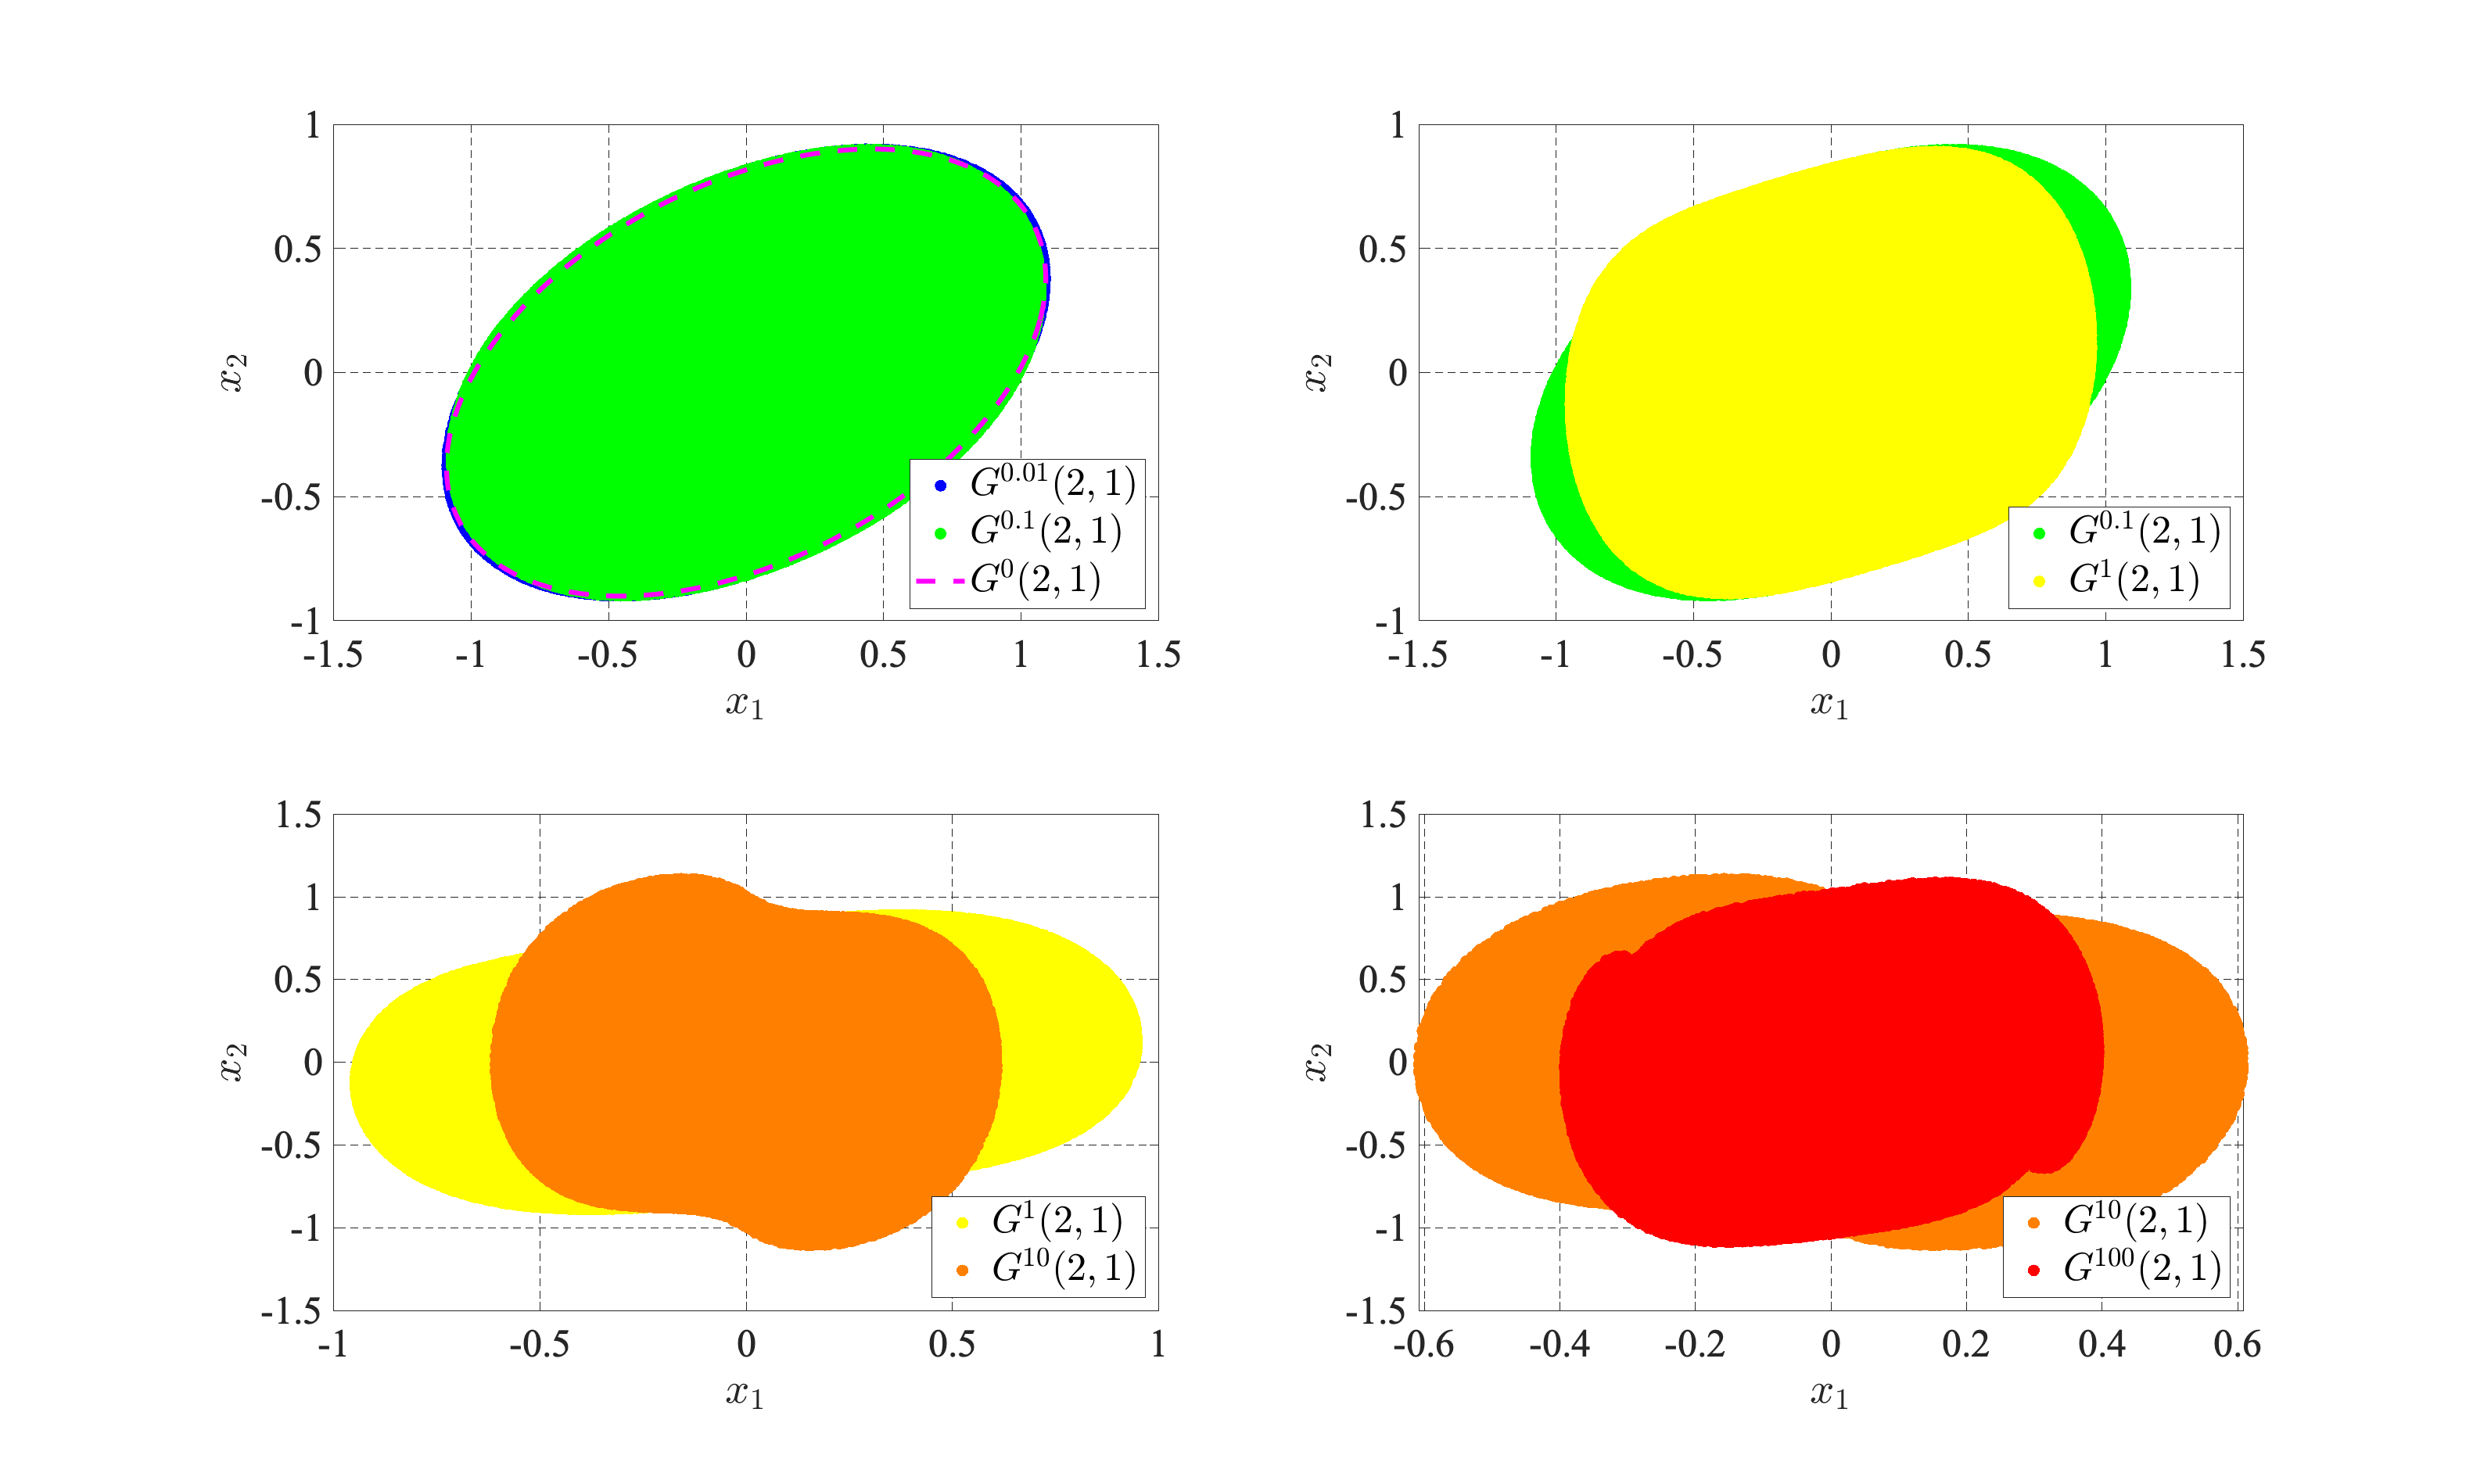
\includegraphics[width=\textwidth]{images/Osipov_QuaziDuffing.eps}}
			\caption{Множества достижимости осциллятора Дуффинга.}
			\label{fig:Duffing}
		\end{figure}
	\end{frame}
	
	\begin{frame}{Пример 2}
		Эта система описывается уравнениями
		\begin{gather}\label{Linear+Dubins}
			\begin{pmatrix} 
				\dot{x}_1 \\
				\dot{x}_2 \\ 
				\dot{x}_3 \end{pmatrix} = 
			\begin{pmatrix}
				0 & 1 & 0 \\
				0 & 0 & 1 \\
				0 & 0 & 0
			\end{pmatrix}
			\begin{pmatrix} 
				x_1 \\
				x_2 \\ 
				x_3 \end{pmatrix} + 
			\varepsilon
			\begin{pmatrix}
				\cos x_3 - x_2\\
				\sin x_3 - x_3 \\
				0
			\end{pmatrix} + 
			\begin{pmatrix}
				0 \\ 0 \\ 1
			\end{pmatrix} u.
		\end{gather}
		При $\varepsilon = 0$, уравнения  \eqref{Linear+Dubins} описывают линейную систему, а при $\varepsilon = 1$ — уницикл. 
		Нелинейный член содержит малый параметр и функцию 
		\begin{gather*}
			f(x) = \begin{pmatrix}
				\cos x_3 - x_2\\
				\sin x_3 - x_3 \\
				0
			\end{pmatrix}.
		\end{gather*}
		
		Начальное состояние $x_1(0) = x_2(0) = x_3(0) = 0 $.\\
		Ограничения на управление такие же, как в первом примере, но интервал времени $0 \leqslant t \leqslant 1$.\\
		Выполнены условия Предположений \ref{s1:as:right_hand_side_conditions_global} и \ref{s1:as:right_hand_side_diff_lip}.
	\end{frame}
	
	\begin{frame}{Пример 2}
		\begin{figure}[ht]
			\centerline{
				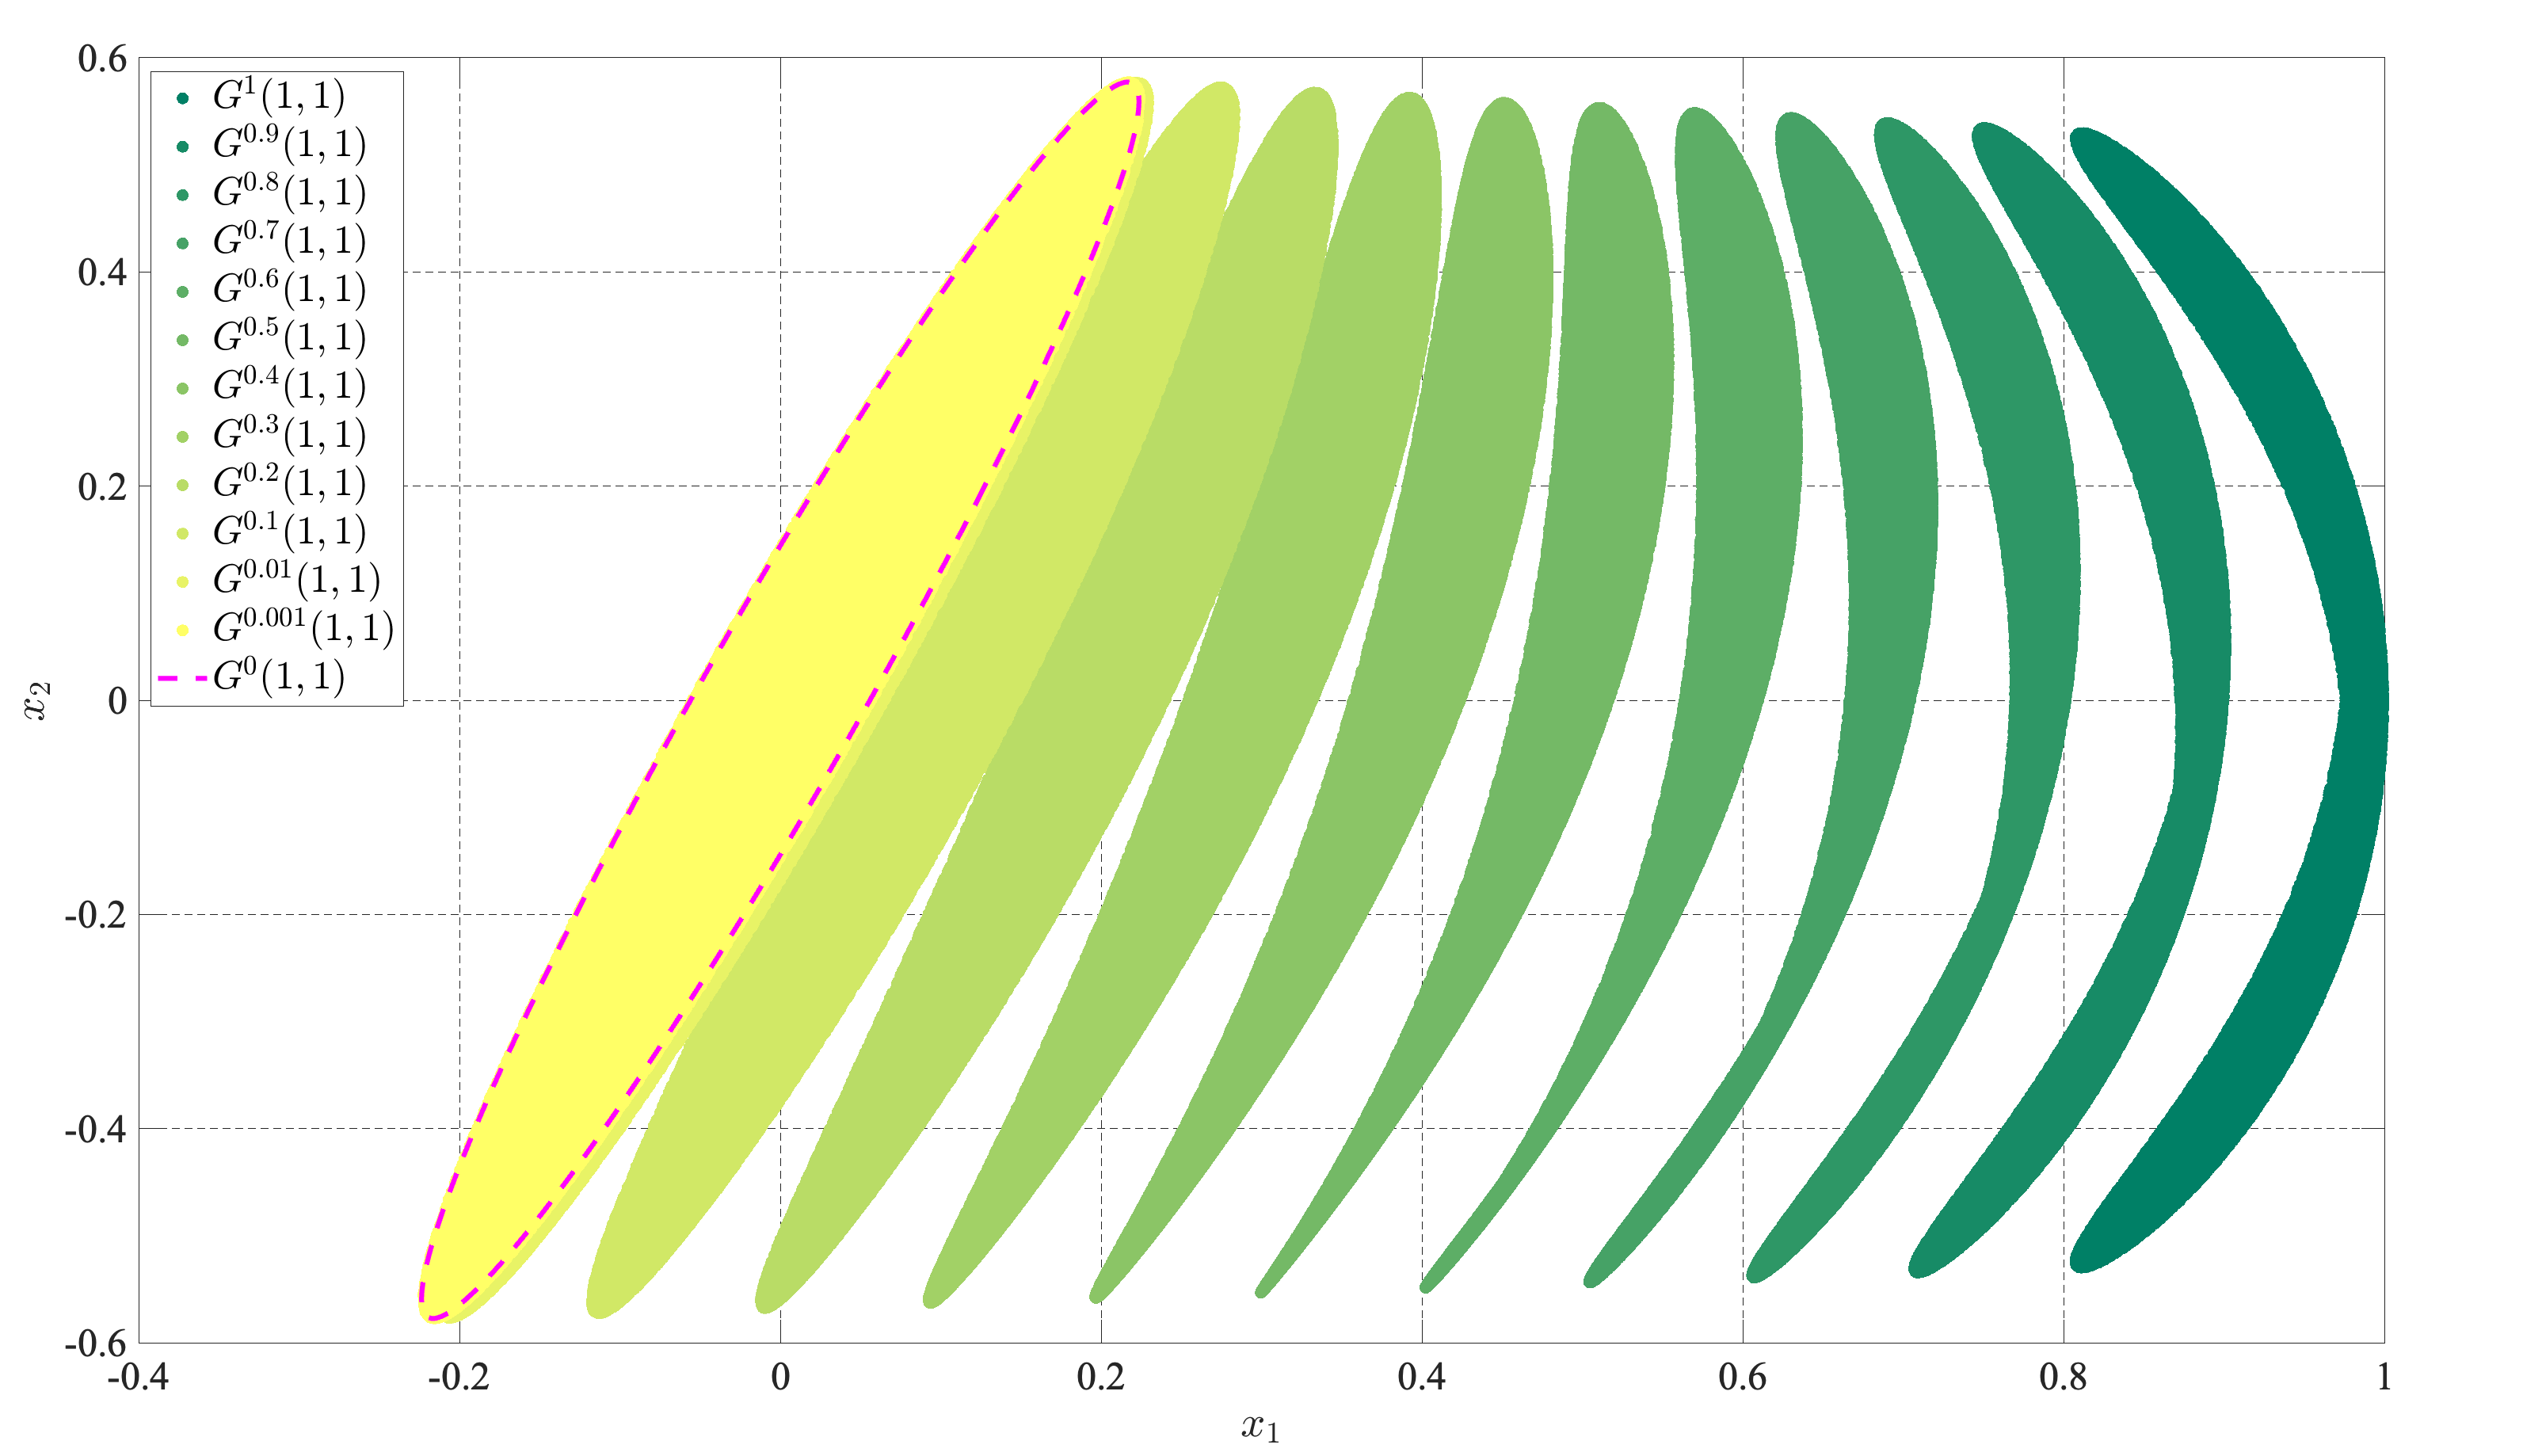
\includegraphics[width=\textwidth]{images/Osipov_QuaziDubins.eps}}
			\caption{Множества достижимости системы \eqref{Linear+Dubins}.}
			\label{fig:LinearDubins}
		\end{figure}
	\end{frame}
	
	\begin{frame}{Пример 3.}
		Рассматривается двумерная нелинейная система
		\begin{gather}\label{Example3}
			\dot{x_1} = x_2, \qquad
			\dot{x_2} = u + \varepsilon(\sin x_1 + \cos x_1) ,\qquad 0\leqslant t  \leqslant 1
		\end{gather}
		Начальное состояние $x_1(0) = x_2(0) = 0 $, управление ограничено  
		\begin{gather}\label{example3_controls}
			\int\limits_0^1 u^2dt \leqslant 1.
		\end{gather}
		При $\varepsilon = 0$, уравнения \eqref{Example3} описывают линейную систему с матрицами
		\begin{gather*}
			A = \begin{pmatrix} 0 & 1\\
				0 & 0
			\end{pmatrix}, \quad B = \begin{pmatrix}
				0\\
				1
			\end{pmatrix}.
		\end{gather*}
		
		Нелинейный член содержит малый параметр и функцию $f(x) = [0; \sin x_1 + \cos \ x_1]$.
	\end{frame}
	
	\begin{frame}{Пример 3.}
		\begin{figure}[t]
			\centerline{
				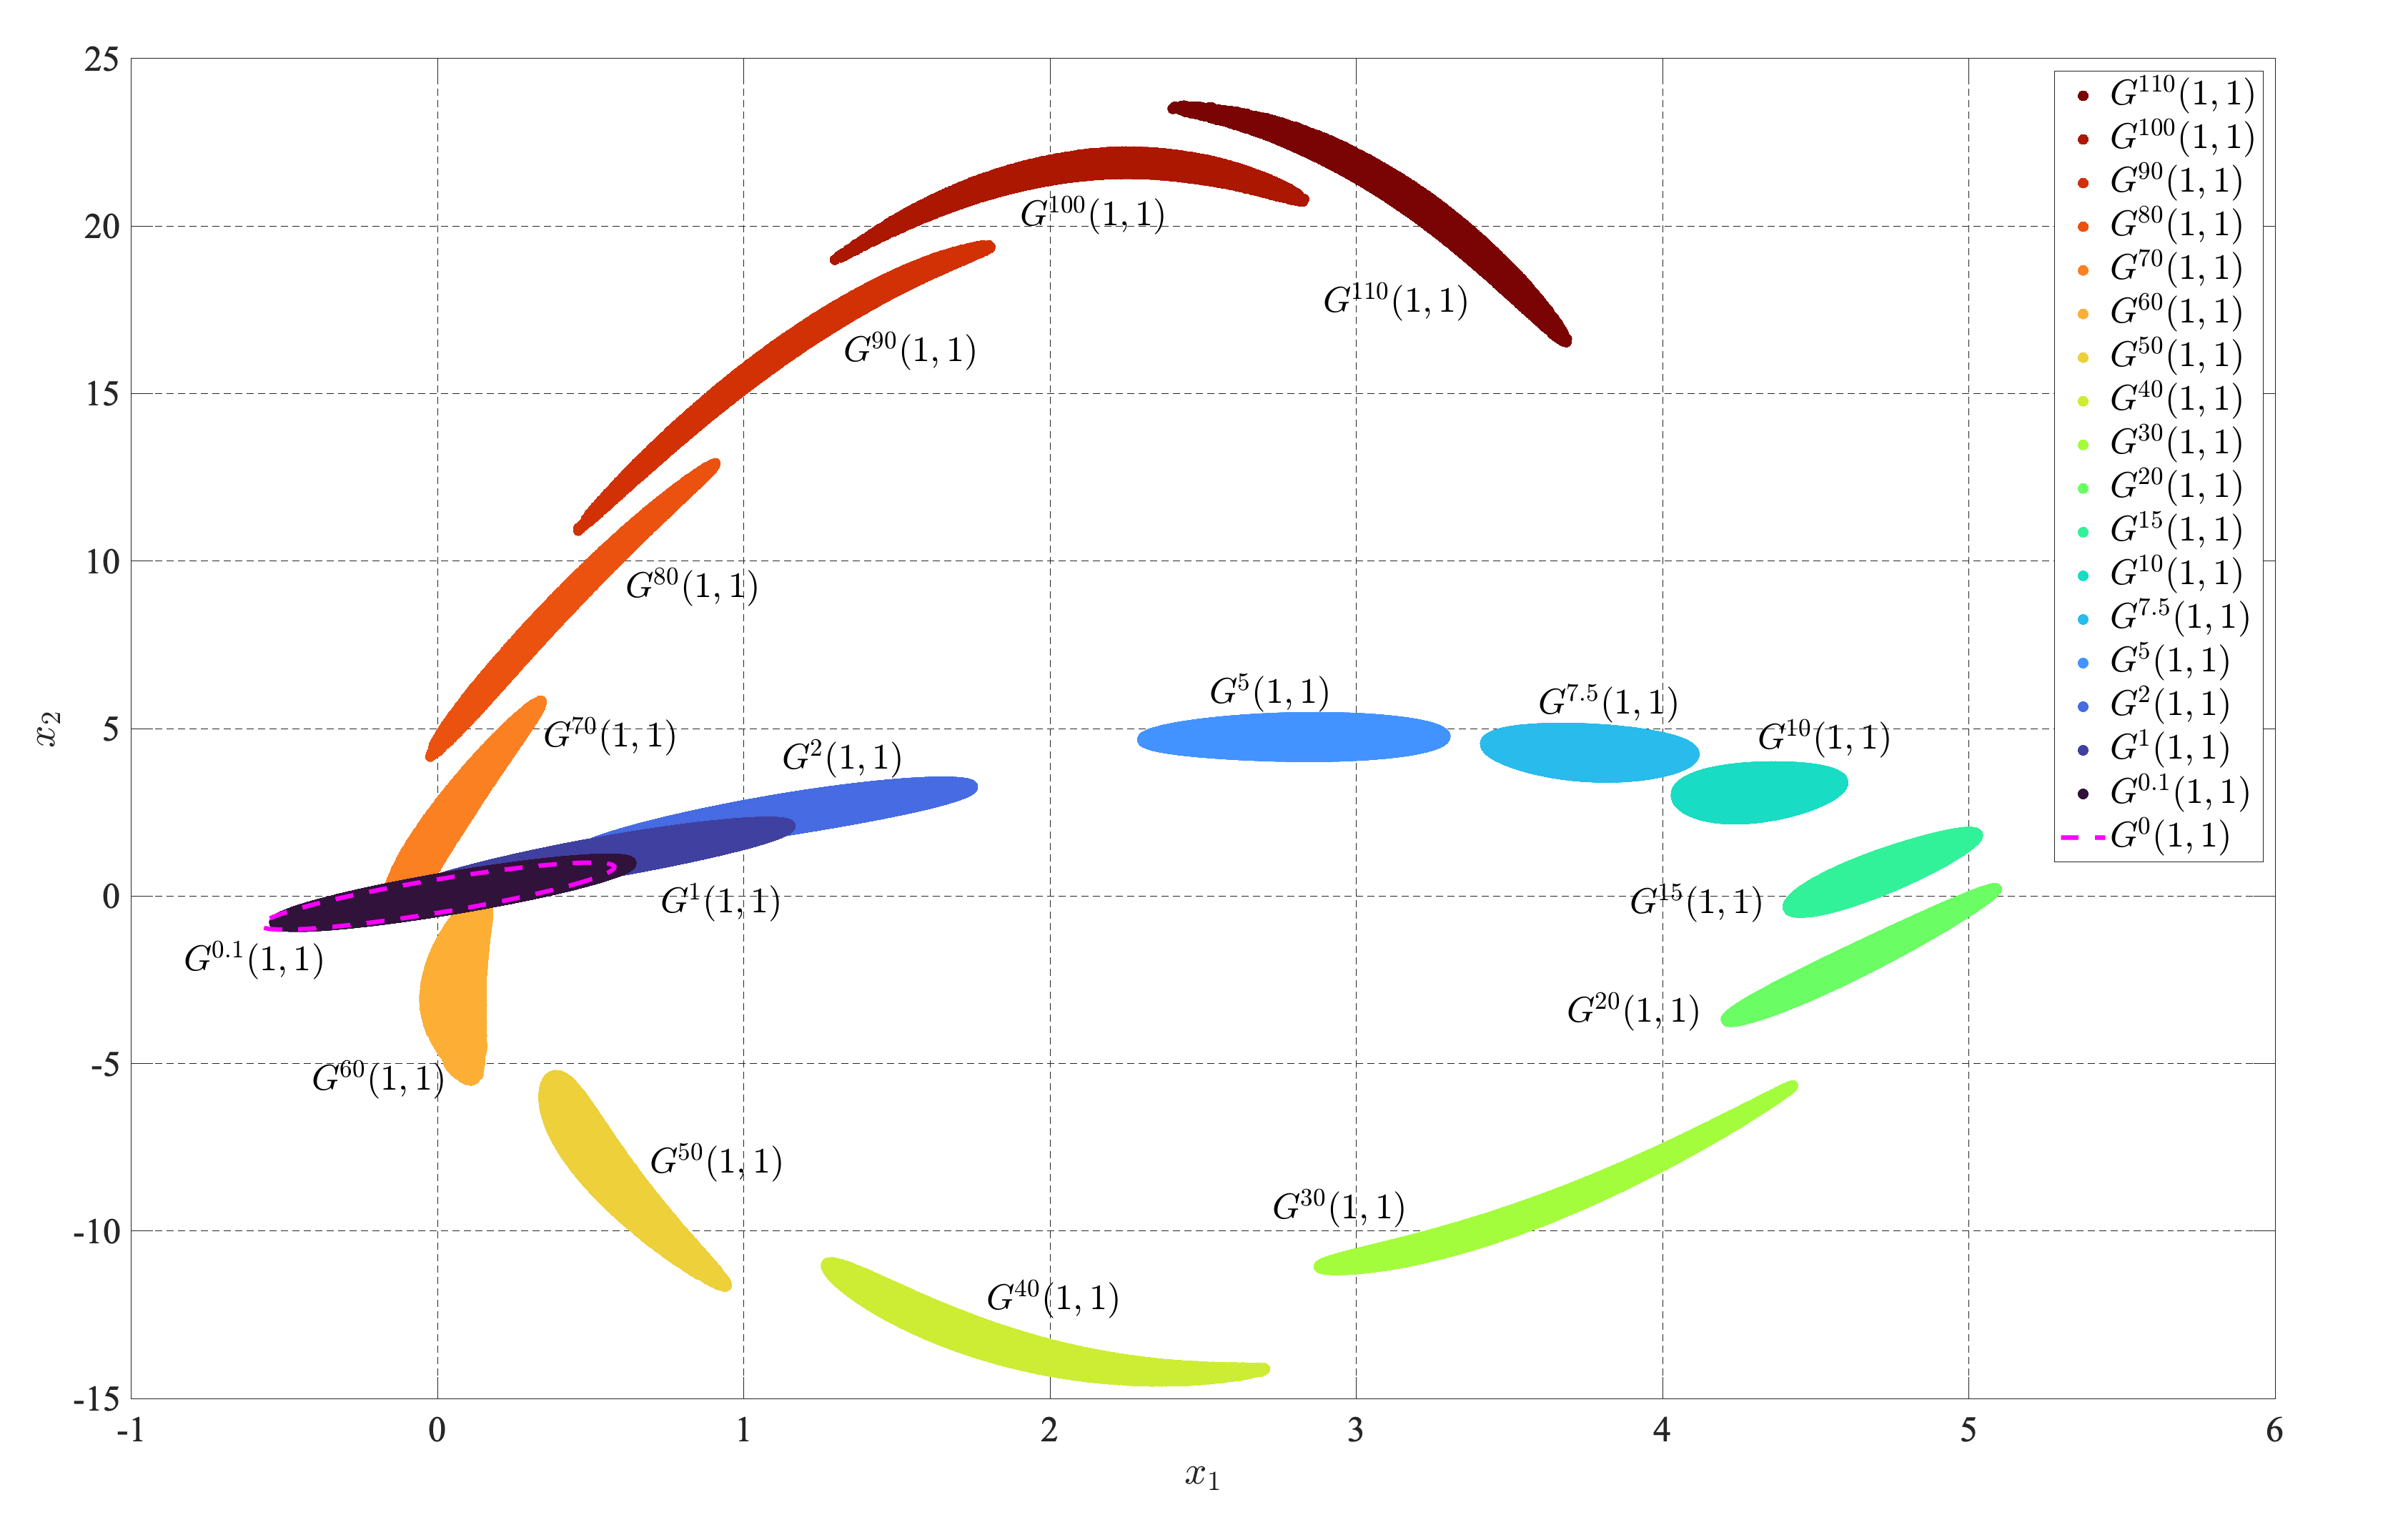
\includegraphics[width=0.92\textwidth]{images/Osipov_QuaziLinearExp.eps}}
			\caption{Множества достижимости системы \eqref{Example3}.}
			\label{fig:Duffing}
		\end{figure}
	\end{frame}

\section{Приложение}

\begin{frame}{Приложение. Численный метод построения множеств достижимости при интегрально-квадратичных ограничениях на управление}
	\begin{columns}
		\begin{column}{0.5\textwidth}
			\begin{itemize}
				\item[\emoji{one}] Перебираем управления $u_i(t) = C_i p(t)$;
				\item[\emoji{two}] Каждое управление порождает решение $ x_i(T, u_i(\cdot)) $;
				\item[\emoji{three}] Результат --- множество $\{x_i(T, u_i(\cdot))\}$;
			\end{itemize}
			\vspace{5mm}
			Управления $u_i(\cdot)$ удовлетворяют ограничениям, если:
			\begin{itemize}
				\item Компоненты $p(t)$, $p: [t_0, {T}] \rightarrow \mathbb{R}^{k+1} $ --- ортонормированный базис в $\mathbb{L}_2[t_0, {T}]$,
				$p(t) = \big(p_{0}(t),p_{1}(t),\dots,p_{k}(t)\big)$,
				$ \langle p_{j}(\cdot), p_{m}(\cdot) \rangle_{\mathbb{L}_2[t_0, {T}]} = 0$, $ j \neq m$; 
				\item $C_i \in \mathbb{R}^{r \times k+1}$ такие, что  $ \|C_i\| \leqslant \mu$;
			\end{itemize}
		\end{column}
		\begin{column}{0.5\textwidth}
			\RestyleAlgo{ruled}
			\begin{algorithm}[H]
				\SetKwFunction{Propagate}{Propagate}
				\SetKwInOut{Parameters}{parameters}\SetKwInOut{Data}{data}\SetKwInOut{Output}{output}
				\Parameters{Number of samples $N$, Degree of polynomial $k$}
				\Data{Control resource $\mu$, Initial condition $x_0$, $t_0$, $T$}
				\Output{$\{x_i\}_{i = 1}^{N}$}
				$p(t) \gets $ Orthonormal polynomials in $\mathbb{L}_2[t,T]$ \;
				\For{$i\leftarrow 0$ \KwTo $N$}{
					$C \gets $ Random matrix from $B_{\mathbb{R}^{r \times k+1}}(0,\mu)$ \;
					$u(t) \gets C p(t)$ \;
					$x_i \gets $ \Propagate$\big(x_0, u(t), t_0, T\big)$\; }
			\end{algorithm}
		\end{column}
	\end{columns}
\end{frame}

\section{.}

\begin{frame}{Положения, выносимые на защиту}
	\begin{itemize}	
		\item[\emoji{one}] Для выпуклых компактов в $\mathbb{R}^n$, зависящих от малого параметра, введено понятие асимптотической эквивалентности, основанное на расстоянии Банаха--Мазура.
		Получены достаточные условия асимптотической эквивалентности множеств достижимости по выходу нелинейных систем с интегрально-квадратичными ограничениями на управление и соответствующих множеств линеаризованных систем. 
		Эти условия совпадают с достаточным условием выпуклости множеств достижимости на малых интервалах времени.
	\end{itemize}
\end{frame}

\begin{frame}{Положения, выносимые на защиту}
	\begin{itemize}			
		\item[\emoji{two}] Исследована задача синтеза управления для нелинейной аффинной по управлению системы с интегрально-квадратичным функционалом. 
		Доказано, что линейная обратная связь, построенная для линеаризованной системы, также обеспечивает локальное решение задачи синтеза для нелинейной системы на достаточно малом промежутке времени. 
		Это требует ограничений на асимптотику грамиана управляемости, которые совпадают с достаточными условиями, обеспечивающими асимптотическую эквивалентность множеств достижимости (множеств нуль-управляемости). 
		В этом случае линейная обратная связь, решающая задачу приведения линеаризованной системы в начало координат за заданное время, будет приводить в начало координат и нелинейную систему из малой окрестности нуля.
		Также при этих условиях получена оценка для относительных значений погрешности интегрального функционала. 
	\end{itemize}
\end{frame}

\begin{frame}{Положения, выносимые на защиту}
	\begin{itemize}	
		\item[\emoji{three}] Для квазилинейных систем с интегральными квадратичными ограничениями на управление исследована выпуклость множеств достижимости. 
		Опираясь на достаточные условия выпуклости образа гильбертова шара при его квазилинейном отображении, доказано, что множества достижимости квазилинейной системы остаются выпуклыми при малых значениях малого параметра. 
	\end{itemize}
\end{frame}

\begin{frame}{Публикации автора по теме диссертации. Публикации в изданиях, рекомендованных ВАК}
	\begin{thebibliography}{11}{\small 
	\bibitem{GusevOsipovTrudy}
	Гусев~М.\,И., Осипов~И.\,О. Асимптотическое поведение множеств достижимости на малых временных промежутках~// Тр. Ин-та математики и механики УрО РАН. --- 2019. --- Т.~25, №~3. --- С.~86--99.
	{\footnotesize ВАК К1; WoS (ESCI), Scopus, MathSciNet, RSCI.}
	\\ Переводная версия: \\
	Gusev~M.\,I., Osipov~I.\,O. Asymptotic behavior of reachable sets on small time intervals~// Proc. Steklov Inst. Math. --- 2020. --- Vol.~309, Suppl.~1. --- P.~S52--S64.
	{\footnotesize WoS(SCIE), Scopus, MathSciNet, Springer.}
	
	%2021
	\bibitem{Osipov}
	Осипов~И.\,О. О выпуклости множеств достижимости по части координат нелинейных управляемых систем на малых промежутках времени~// Вестник Удмуртского университета. Математика. Механика. Компьютерные науки. --- 2021. --- Т.~31, вып.~2. --- C.~210--225.
	{\footnotesize  ВАК; К1: WoS (ESCI), Scopus, MathSciNet, zbMATH, RSCI.}
	
	%2021 
	\bibitem{Voronezh}
	Осипов~И.\,О. Об асимптотике собственных чисел грамиана управляемости линейной системы с малым параметром~// Итоги науки и техники. Сер. Соврем. математика и eё прил. Темат. обзоры. --- 2021. --- Т.~191. --- С.~115--122.
	{\footnotesize ВАК; К1: MathSciNet.}
	\\Переводная версия: \\
	Osipov~I.\,O. On the Asymptotics of Eigenvalues of the Controllability Gramian of a Linear System with a Small Parameter~// J. Math. Sci. --- 2025. --- Vol.~288. --- P.~780--787. 
	{\footnotesize К1: Scopus, zbMATH, Springer.} }
	\end{thebibliography}
\end{frame}

\begin{frame}{Публикации автора по теме диссертации. Публикации в изданиях, рекомендованных ВАК}
	\begin{thebibliography}{11}{\small 			
			%2022
			\bibitem{GusevOsipov} 
			Гусев~М.\,И., Осипов~И.\,О. О задаче локального синтеза для нелинейных систем с интегральными ограничениями~// Вестник Удмуртского университета. Математика. Механика. Компьютерные науки. --- 2022. --- Т.~32, №~2. --- С.~171--186. 
			{\footnotesize ВАК; К1: WoS (ESCI), Scopus, MathSciNet, zbMATH, RSCI.}
			
			
			%2023
			\bibitem{OsipovUMJ}
			Osipov~I.\,O. Convexity of Reachable Sets of Quasilinear Systems~// Ural Math. J. --- 2023. --- Vol.~9, no.~2. --- P.~141--156.
			{\footnotesize ВАК; К1: Scopus, MathSciNet, zbMATH, RSCI.} }
	\end{thebibliography}
\end{frame}

\begin{frame}{Публикации автора по теме диссертации. Другие публикации, включенные в международные базы данных}
	\begin{thebibliography}{11}{\small 			
		%2019
		\bibitem{AIP}
		Gusev~M.\,I., Osipov~I.\,O. On Convexity of Small-time Reachable Sets of Nonlinear Control Systems~// AIP Conference Proceedings. --- 2019. --- Vol.~2164. --- Art.~no.~060007.
		{\footnotesize WoS, Scopus. }
		
		%2022
		\bibitem{GusevOsipovPyat}
		Gusev~M., Osipov~I. On Local Control Synthesis for Nonlinear Systems under Integral Constraints~// 2022 16th International Conference on Stability and Oscillations of Nonlinear Control Systems (Pyatnitskiy's Conference), Moscow, 2022. --- P.~1--4.
		{\footnotesize Scopus.}
		
		%2023
		\bibitem{GusevOsipovMotor}
		Gusev~M., Osipov~I. Approximate Solution of Small-Time Control Synthesis Problem Based on Linearization~// Mathematical Optimization Theory and Operations Research. MOTOR 2023. --- Cham~: Springer, 2023. --- (Lecture Notes in Computer Science~; vol.~13930). --- P.~362--377.
		{\footnotesize  zbMATH, MathSciNet, Springer.}
		}
	\end{thebibliography}
\end{frame}

\begin{frame}{Публикации автора по теме диссертации. Свидетельства о государственной регистрации программ для ЭВМ}
	\begin{thebibliography}{11}{\small 			
			%2019
\bibitem{Patent} 
Программа для построения методом Монте-Карло множеств достижимости нелинейных систем с интегральными ограничениями на управление~: свидетельство о~гос. регистрации программы для ЭВМ №~2020661557 ~/~И.\,В.~Зыков, И.\,О.~Осипов~; правообладатель ИММ УрО РАН // Федеральная служба по интеллектуальной собственности (РосПатент) --- Зарег. 24.09.2020. --- URL: https://www.elibrary.ru/item.asp?id=44104691 (дата обращения: 07.09.2025).
		}
	\end{thebibliography}
\end{frame}

\begin{frame}{Конференции}
	\begin{itemize}
		\item Воронежская весенняя математическая школа <<Современные методы теории краевых задач. Понтрягинские чтения–XXX>>, Воронеж, 3 -- 9 мая 2019 г.;
		\item Application of Mathematics in Technical and Natural Sciences \\ (AMiTaNS'11): 11th Intern. Conf., June 20 -- 25, 2019, Albena, Bulgaria;
		\item 51-я, 52-я, 53-я, 54-я и 55-я Международные молодежные школы-конференции "Современные проблемы математики и ее приложений" (2020, 2021, 2022, 2023, 2024), Екатеринбург;
		\item III международный семинар, посвященный 75-летию академика А.\,И.~Субботина, Екатеринбург, 26 -- 30 октября 2020 г.;
		\item Динамические системы: устойчивость, управление, оптимизация: материалы Междунар. науч. конф. памяти Р.\,Ф.~Габасова, Минск, 5 -- 10 окт. 2021 г.;
		\item XVI Международная конференция «Устойчивость и колебания нелинейных систем управления» (конференция Пятницкого), Москва, 1 -- 3 июня 2022 г.;
		\item Теория оптимального управления и приложения (OCTA 2022), Екатеринбург, 27 июня -- 1 июля 2022 г.;
		\item 7-я Международная школа-семинар «Нелинейный анализ и экстремальные задачи» (NLA-2022), 15 -- 22 июля 2022 г., Иркутск;
	\end{itemize}
\end{frame}

\begin{frame}{Конференции}
	\begin{itemize}
		\item 22nd International Conference Mathematical Optimization Theory and Operations Research (MOTOR 2023) Dedicated to 90th Anniversary of Academician I.\,I.~Eremin July 2 -- 8, 2023, Ekaterinburg;
		\item ВСПУ XIV Всероссийское совещание по проблемам управления, Россия, Москва, ИПУ РАН, 17 -- 20 июня 2024 г.;
		\item Международная конференция «Динамические системы: устойчивость, управление, дифференциальные игры» (SCDG2024), посвященная 100-летию со дня рождения академика Н.\,Н.~Красовского, 9 сентября 2024 г. -- 13 сентября 2024 г., г. Екатеринбург;
		\item Современные проблемы математики и eё приложений. Международная (56-я Всероссийская) молодежная школа-конференция памяти ученого и учителя Александра Георгиевича Гейна (29.01.1950 – 23.01.2025) 2 февраля 2025 г. -- 18 февраля 2025 г., г. Екатеринбург;
	\end{itemize}
\end{frame}

	
\end{document}